%& --translate-file=cp1250pl.tcx  %%%%%%%%%%%%%%
%% ----------------------------------------------------------------
%% Thesis.tex -- MAIN FILE (the one that you compile with LaTeX)
%% ---------------------------------------------------------------- 

% Set up the document
\documentclass[a4paper, 11pt, oneside]{Thesis}  % Use the "Thesis" style, based on the ECS Thesis style by Steve Gunn
\graphicspath{{Figures/}}  % Location of the graphics files (set up for graphics to be in PDF format)
\usepackage{polski}

% Include any extra LaTeX packages required
\usepackage[square, numbers, comma, sort&compress]{natbib}  % Use the "Natbib" style for the references in the Bibliography
\usepackage{verbatim}  % Needed for the "comment" environment to make LaTeX comments
\usepackage{vector}  % Allows "\bvec{}" and "\buvec{}" for "blackboard" style bold vectors in maths
\hypersetup{urlcolor=blue, colorlinks=true}  % Colours hyperlinks in blue, but this can be distracting if there are many links.
%% ----------------------------------------------------------------
\begin{document}
\frontmatter	  % Begin Roman style (i, ii, iii, iv...) page numbering

% Set up the Title Page
\title  {Projekt i implementacja aplikacji realizuj�cej operacje arytmetyczne na kwantyfikatorach lingwistycznych}
\authors  {\texorpdfstring
            {\href{btaczala@wi.ps.pl}{Bartosz Tacza�a}}
            {Bartosz Tacza�a}
            }
\addresses  {\groupname\\\deptname\\\univname}  % Do not change this here, instead these must be set in the "Thesis.cls" file, please look through it instead
\date       {\today}
\subject    {}
\keywords   {}

\maketitle
%% ----------------------------------------------------------------

\setstretch{1.3}  % It is better to have smaller font and larger line spacing than the other way round

% Define the page headers using the FancyHdr package and set up for one-sided printing
\fancyhead{}  % Clears all page headers and footers
\rhead{\thepage}  % Sets the right side header to show the page number
\lhead{}  % Clears the left side page header

\pagestyle{fancy}  % Finally, use the "fancy" page style to implement the FancyHdr headers

%% ----------------------------------------------------------------
% Declaration Page required for the Thesis, your institution may give you a different text to place here
\Declaration{

\addtocontents{toc}{\vspace{1em}}  % Add a gap in the Contents, for aesthetics

I, AUTHOR NAME, declare that this thesis titled, `THESIS TITLE' and the work presented in it are my own. I confirm that:

\begin{itemize} 
\item[\tiny{$\blacksquare$}] This work was done wholly or mainly while in candidature for a research degree at this University.
 
\item[\tiny{$\blacksquare$}] Where any part of this thesis has previously been submitted for a degree or any other qualification at this University or any other institution, this has been clearly stated.
 
\item[\tiny{$\blacksquare$}] Where I have consulted the published work of others, this is always clearly attributed.
 
\item[\tiny{$\blacksquare$}] Where I have quoted from the work of others, the source is always given. With the exception of such quotations, this thesis is entirely my own work.
 
\item[\tiny{$\blacksquare$}] I have acknowledged all main sources of help.
 
\item[\tiny{$\blacksquare$}] Where the thesis is based on work done by myself jointly with others, I have made clear exactly what was done by others and what I have contributed myself.
\\
\end{itemize}
 
 
Signed:\\
\rule[1em]{25em}{0.5pt}  % This prints a line for the signature
 
Date:\\
\rule[1em]{25em}{0.5pt}  % This prints a line to write the date
}
\clearpage  % Declaration ended, now start a new page

%% ----------------------------------------------------------------
% The "Funny Quote Page"
\pagestyle{empty}  % No headers or footers for the following pages

\null\vfill
% Now comes the "Funny Quote", written in italics
\textit{``Write a funny quote here.''}

\begin{flushright}
If the quote is taken from someone, their name goes here
\end{flushright}

\vfill\vfill\vfill\vfill\vfill\vfill\null
\clearpage  % Funny Quote page ended, start a new page
%% ----------------------------------------------------------------

% The Abstract Page
\addtotoc{Abstract}  % Add the "Abstract" page entry to the Contents
\abstract{
\addtocontents{toc}{\vspace{1em}}  % Add a gap in the Contents, for aesthetics

The Thesis Abstract is written here (and usually kept to just this page). The page is kept centered vertically so can expand into the blank space above the title too\ldots

}

\clearpage  % Abstract ended, start a new page
%% ----------------------------------------------------------------

\setstretch{1.3}  % Reset the line-spacing to 1.3 for body text (if it has changed)

% The Acknowledgements page, for thanking everyone
\acknowledgements{
\addtocontents{toc}{\vspace{1em}}  % Add a gap in the Contents, for aesthetics

The acknowledgements and the people to thank go here, don't forget to include your project advisor\ldots

}
\clearpage  % End of the Acknowledgements
%% ----------------------------------------------------------------

\pagestyle{fancy}  %The page style headers have been "empty" all this time, now use the "fancy" headers as defined before to bring them back


%% ----------------------------------------------------------------
\lhead{\emph{Contents}}  % Set the left side page header to "Contents"
\tableofcontents  % Write out the Table of Contents

%% ----------------------------------------------------------------
\lhead{\emph{List of Figures}}  % Set the left side page header to "List if Figures"
\listoffigures  % Write out the List of Figures

%% ----------------------------------------------------------------
\lhead{\emph{List of Tables}}  % Set the left side page header to "List of Tables"
\listoftables  % Write out the List of Tables

%% ----------------------------------------------------------------
\setstretch{1.5}  % Set the line spacing to 1.5, this makes the following tables easier to read
\clearpage  % Start a new page
\lhead{\emph{Abbreviations}}  % Set the left side page header to "Abbreviations"
\listofsymbols{ll}  % Include a list of Abbreviations (a table of two columns)
{
% \textbf{Acronym} & \textbf{W}hat (it) \textbf{S}tands \textbf{F}or \\
\textbf{LAH} & \textbf{L}ist \textbf{A}bbreviations \textbf{H}ere \\

}

%% ----------------------------------------------------------------
\clearpage  % Start a new page
\lhead{\emph{Physical Constants}}  % Set the left side page header to "Physical Constants"
\listofconstants{lrcl}  % Include a list of Physical Constants (a four column table)
{
% Constant Name & Symbol & = & Constant Value (with units) \\
Speed of Light & $c$ & $=$ & $2.997\ 924\ 58\times10^{8}\ \mbox{ms}^{-\mbox{s}}$ (exact)\\

}

%% ----------------------------------------------------------------
\clearpage  %Start a new page
\lhead{\emph{Symbols}}  % Set the left side page header to "Symbols"
\listofnomenclature{lll}  % Include a list of Symbols (a three column table)
{
% symbol & name & unit \\
$a$ & distance & m \\
$P$ & power & W (Js$^{-1}$) \\
& & \\ % Gap to separate the Roman symbols from the Greek
$\omega$ & angular frequency & rads$^{-1}$ \\
}
%% ----------------------------------------------------------------
% End of the pre-able, contents and lists of things
% Begin the Dedication page

\setstretch{1.3}  % Return the line spacing back to 1.3

\pagestyle{empty}  % Page style needs to be empty for this page
\dedicatory{For/Dedicated to/To my\ldots}

\addtocontents{toc}{\vspace{2em}}  % Add a gap in the Contents, for aesthetics


%% ----------------------------------------------------------------
\mainmatter	  % Begin normal, numeric (1,2,3...) page numbering
\pagestyle{fancy}  % Return the page headers back to the "fancy" style

% Include the chapters of the thesis, as separate files
% Just uncomment the lines as you write the chapters

% Wprowadzenie, rozdzia� 1 
\chapter{Wprowadzenie} 
\label{Rozdzia� 1 }
\lhead{Rozdzia� 1. \emph{Wprowadzenie }} % Write in your own chapter title to set the page header


\section{Welcome and Thank You}

Welcome to this ``\LaTeX{} Thesis Template'', a beautiful and easy to use template for writing a thesis using the \LaTeX{} typesetting system.

If you are writing a thesis (or will be in the future) and its subject is technical or mathematical (though it doesn't have to be), then creating it in \LaTeX{} is highly recommended as a way to make sure you can just get down to the essential writing without having to worry over formatting or wasting time arguing with your word processor.

\LaTeX{} is easily able to professionally typeset documents that run to hundreds or thousands of pages long. With simple mark-up commands, it automatically sets out the table of contents, margins, page headers and footers and keeps the formatting consistent and beautiful. One of its main strengths is the way it can easily typeset mathematics, even \emph{heavy} mathematics. Even if those equations are the most horribly twisted and most difficult mathematical problems that can only be solved on a super-computer, you can at least count on \LaTeX{} to make them look stunning.

\subsection{Examples of \LaTeX{} Typeset eBooks}

You can see (and download and read) examples of eBooks typeset by \LaTeX{} in a small library here:\\
\href{http://www.sunilpatel.co.uk/typesetting.html}{\texttt{http://www.sunilpatel.co.uk/typesetting.html}}

The books are available for you to download for free. They were originally plain text files but were quickly and easily converted into beautifully typeset and well presented eBooks through \LaTeX{} for you to enjoy.


\section{Learning \LaTeX{}}

\LaTeX{} is not a WYSIWYG (What You See is What You Get) program, unlike word processors such as Microsoft Word or Corel WordPerfect. Instead, a document written for \LaTeX{} is actually a simple, plain text file that contains \emph{no formatting}. You tell \LaTeX{} how you want the formatting in the finished document by writing in simple commands amongst the text, for example, if I want to use \emph{italic text for emphasis}, I write the `$\backslash$\texttt{emph}\{\}' command and put the text I want in italics in between the curly braces. This means that \LaTeX{} is a ``mark-up'' language, very much like HTML.

\subsection{A (not so short) Introduction to \LaTeX{}}

If you are new to \LaTeX{}, there is a very good eBook -- freely available online as a PDF file -- called, ``The Not So Short Introduction to \LaTeX{}''. The book's title is typically shortened to just ``lshort''. You can download the latest version (as it is occasionally updated) from here:\\
\href{http://www.ctan.org/tex-archive/info/lshort/english/lshort.pdf}{\texttt{http://www.ctan.org/tex-archive/info/lshort/english/lshort.pdf}}

It is also available in several other languages. Find yours from the list on this page:\\
\href{http://www.ctan.org/tex-archive/info/lshort/}{\texttt{http://www.ctan.org/tex-archive/info/lshort/}}

It is recommended to take a little time out to learn how to use \LaTeX{} by creating several, small `test' documents. Making the effort now means you're not stuck learning the system when what you \emph{really} need to be doing is writing your thesis.

\subsection{A Short Math Guide for \LaTeX{}}

If you are writing a technical or mathematical thesis, then you may want to read the document by the AMS (American Mathematical Society) called, ``A Short Math Guide for \LaTeX{}''. It can be found online here:\\
\href{http://www.ams.org/tex/amslatex.html}{\texttt{http://www.ams.org/tex/amslatex.html}}\\
under the ``Additional Documentation'' section towards the bottom of the page.

\subsection{Common \LaTeX{} Math Symbols}
There are a multitude of mathematical symbols available for \LaTeX{} and it would take a great effort to learn the commands for them all. The most common ones you are likely to use are shown on this page:\\
\href{http://www.sunilpatel.co.uk/latexsymbols.html}{\texttt{http://www.sunilpatel.co.uk/latexsymbols.html}}

You can use this page as a reference or crib sheet, the symbols are rendered as large, high quality images so you can quickly find the \LaTeX{} command for the symbol you need.

\subsection{\LaTeX{} on a Mac}
 
The \LaTeX{} package is available for many systems including Windows, Linux and Mac OS X. The package for OS X is called MacTeX� and it contains all the applications you need � bundled together and pre-customised � for a fully working \LaTeX{} environment and work�ow.
 
MacTeX includes a dedicated \LaTeX{} IDE (Integrated Development Environment) called ``TeXShop'' for writing your `\texttt{.tex}' files and ``BibDesk'': a program to manage your references and create your bibliography section just as easily as managing songs and creating playlists in iTunes. To learn more about using \LaTeX{} on the Mac system, read the guide at:\\
\href{http://www.sunilpatel.co.uk/texhelp.html}{\texttt{http://www.sunilpatel.co.uk/texhelp.html }}


\section{Getting Started with this Template}

If you are familiar with \LaTeX{}, then you can familiarise yourself with the contents of the \href{http://www.sunilpatel.co.uk/files/Thesis\%20Template.zip}{Zip file} and the directory structure and then place your own information into the `\texttt{Thesis.cls}' file. Section \ref{FillingFile} on page \pageref{FillingFile} tells you how to do this. Make sure you read section \ref{ThesisConventions} about thesis conventions to get the most out of this template and then get started with the `\texttt{Thesis.tex}' file straightaway.

If you are new to \LaTeX{} it is recommended that you carry on reading through the rest of the information in this document.

\subsection{Latest Version}

This thesis template you have downloaded is version 1.2 and you can always find the latest version of this template online at:\\
\href{http://www.sunilpatel.co.uk/thesistemplate.html}{\texttt{http://www.sunilpatel.co.uk/thesistemplate.html}}

\subsection{List of Changes}

\subsubsection*{Version 1.2 (March 2008)}

This is version 1.2 and contains more corrections, improved advice on figures, an additional section for users on Mac systems and a major correction for those wishing to use US Letter sized paper for their thesis.

\subsubsection*{Version 1.1.2 (August 2007)}
This is version 1.1.2 and contains trivial (language and spelling) corrections.

\subsubsection*{Version 1.1.1 (May 2007)}
This is version 1.1.1 and corrects (updates) several hyperlinks that have changed. The file ``\texttt{lstpatch.sty}'' is also included as some \TeX{} distributions do not include it.

\subsubsection*{Version 1.1 (April 2007)}
This is version 1.1, released shortly after 1.0. It contains \emph{lots} of general text corrections (spelling, punctuation and grammar) and includes a link to a page containing a list of common \LaTeX{} math symbols, available at:\\
\href{http://www.sunilpatel.co.uk/latexsymbols.html}{\texttt{http://www.sunilpatel.co.uk/latexsymbols.html}}


\subsubsection*{Version 1.0 (March 2007)}
This is the first version, released to the public in March 2007.

\subsection{About this Template}

This \LaTeX{} Thesis Template is originally based and created around a \LaTeX{} style file created by Steve R.\ Gunn from the University of Southampton (UK), department of Electronics and Computer Science. You can find his original thesis style file at his site, here:\\
\href{http://www.ecs.soton.ac.uk/~srg/softwaretools/document/templates/}{\texttt{http://www.ecs.soton.ac.uk/$\sim$srg/softwaretools/document/templates/}}

My thesis originally used the `\texttt{ecsthesis.cls}' from his list of styles. However, I knew \LaTeX{} could still format better. To get the look I wanted, I modified his style and also created a skeleton framework and folder structure to place the thesis files in.

This Thesis Template consists of that modified style, the framework and the folder structure. All the work that has gone into the preparation and groundwork means that all you have to bother about is the writing.

Some of the modifications made to the original template include:
\begin{itemize}
\item Addition of the, `Declaration of Authorship' page
\item Optimised page layout for one-sided printing
\item Better page headers (changed from the default headers)
\item Full bibliography information (with `\texttt{natbib}' and `\texttt{unsrtnat}') that numerically sorts and compresses multiple references and also includes the URL field (with an active link) and DOI information if supplied
\item Change of font size and line spacing to increase readability
\item Added, `List of Symbols' page
\item Added, `funny quote' page
\end{itemize}


Before you begin using this template you should ensure that its style complies with the thesis style guidelines imposed by your institution. As this template is based on the style for the University of Southampton (UK), it can definitely be used without modification for Southampton PhD theses.

In most cases this template style and layout will be suitable. If it is not, it may only require a small change to bring the template in line with your institution's recommendations.


\section{What this Template Includes}

\subsection{Folders}

This template comes as a single \href{http://www.sunilpatel.co.uk/files/Thesis\%20Template.zip}{Zip file} that expands out to many files and folders. The folder names are mostly self-explanatory:

\textbf{Appendices} -- this is the folder where you put the appendices. Each appendix should go into its own separate `\texttt{.tex}' file.

\textbf{Chapters} -- this is the folder where you put the thesis chapters. A thesis usually has about seven chapters, though there is no hard rule on this. Each chapter should go in its own separate `\texttt{.tex}' file and they usually are split as:
\begin{itemize}
\item Chapter 1: Introduction to the thesis topic
\item Chapter 2: Background information and theory
\item Chapter 3: (Laboratory) experimental setup
\item Chapter 4: Details of experiment 1
\item Chapter 5: Details of experiment 2
\item Chapter 6: Discussion of the experimental results
\item Chapter 7: Conclusion and future directions
\end{itemize}
This chapter layout is specialised for the experimental sciences.

\textbf{Figures} -- this folder contains the all figures for the thesis. These are the final images that will go into the thesis document.

\textbf{Primitives} -- this is the folder that contains scraps, particularly because one final image in the `Figures' folder may be made from many separate images and photos, these source images go here. This keeps the intermediate files separate from the final thesis figures.

\subsection{Files}

Included are also several files, most of them are plain text and you can see their contents in a text editor. Luckily, many of them are auxiliary files created by \LaTeX{} or BibTeX and which you don't need to bother about:

\textbf{Bibliography.bib} -- this is an important file that contains all the bibliographic information and references that you will be citing in the thesis for use with BibTeX. You can write it manually, but there are reference manager programs available that will create and manage it for you. Bibliographies in \LaTeX{} are a large subject and you may need to read about BibTeX before starting with this.

\textbf{Thesis Todo List.txt} -- this is a Todo list that provides a simple way to track the thesis progress and also helps you see what parts need attention. Inside is a structured layout for you to enter all this information. Do not try to fill it out all at once, but write the tasks in as you come across them i.e.\ write an entry for a figure that needs creating only when you refer to or write about it (and hence need to place it) in the thesis text.

\textbf{Thesis.cls} -- this is an important file. It is the style file that tells \LaTeX{} how to format the thesis. You will also need to open this file in a text editor and fill in your own information (such as name, department, institution). Luckily, this is not too difficult and is explained in section \ref{FillingFile} on page \pageref{FillingFile}.

\textbf{Thesis.pdf} -- this is your beautifully typeset thesis (in the PDF file format) created by \LaTeX{}.

\textbf{Thesis.tex} -- this is an important file. This is the file that you tell \LaTeX{} to compile to produce your thesis as a PDF file. It contains the framework and constructs that tell \LaTeX{} how to layout the thesis. It is heavily commented so you can read exactly what each line of code does and why it is there. After you put your own information into the `\texttt{Thesis.cls}' file, go to this file and begin filling it in -- you have now started your thesis!

\textbf{vector.sty} -- this is a \LaTeX{} package, it tells \LaTeX{} how to typeset mathematical vectors. Using this package is very easy and you can read the documentation on the site (you just need to look at the `\texttt{vector.pdf}' file):\\
\href{http://www.ctan.org/tex-archive/macros/latex/contrib/vector/}{\texttt{http://www.ctan.org/tex-archive/macros/latex/contrib/vector/}}

\textbf{lstpatch.sty} -- this is a \LaTeX{} package required by this LaTeX template and is included as not all \TeX{} distributions have it installed by default. You do not need to modify this file.

Files that are \emph{not} included, but are created by \LaTeX{} as auxiliary files include:

\textbf{Thesis.aux} -- this is an auxiliary file generated by \LaTeX{}, if it is deleted \LaTeX{} simply regenerates it when you run the main `\texttt{.tex}' file.

\textbf{Thesis.bbl} -- this is an auxiliary file generated by BibTeX, if it is deleted, BibTeX simply regenerates it when you run the main tex file. Whereas the `\texttt{.bib}' file contains all the references you have, this `\texttt{.bbl}' file contains the references you have actually cited in the thesis and is used to build the bibliography section of the thesis.

\textbf{Thesis.blg} -- this is an auxiliary file generated by BibTeX, if it is deleted BibTeX simply regenerates it when you run the main `\texttt{.tex}' file.

\textbf{Thesis.lof} -- this is an auxiliary file generated by \LaTeX{}, if it is deleted \LaTeX{} simply regenerates it when you run the main `\texttt{.tex}' file. It tells \LaTeX{} how to build the `List of Figures' section.

\textbf{Thesis.log} -- this is an auxiliary file generated by \LaTeX{}, if it is deleted \LaTeX{} simply regenerates it when you run the main `\texttt{.tex}' file. It contains messages from \LaTeX{}, if you receive errors and warnings from \LaTeX{}, they will be in this `\texttt{.log}' file.

\textbf{Thesis.lot} -- this is an auxiliary file generated by \LaTeX{}, if it is deleted \LaTeX{} simply regenerates it when you run the main `\texttt{.tex}' file. It tells \LaTeX{} how to build the `List of Tables' section.

\textbf{Thesis.out} -- this is an auxiliary file generated by \LaTeX{}, if it is deleted \LaTeX{} simply regenerates it when you run the main `\texttt{.tex}' file.


So from this long list, only the files with the `\texttt{.sty}', `\texttt{.bib}', `\texttt{.cls}' and `\texttt{.tex}' extensions are the most important ones. The other auxiliary files can be ignored or deleted as \LaTeX{} and BibTeX will regenerate them.


\section{Filling in the `\texttt{Thesis.cls}' File}\label{FillingFile}

You will need to personalise the thesis template and make it your own by filling in your own information. This is done by editing the `\texttt{Thesis.cls}' file in a text editor.

Open the file and scroll down, past all the `$\backslash$\texttt{newcommand}\ldots' items until you see the entries for `\texttt{University Name}', `\texttt{Department Name}', etc\ldots.

Fill out the information about your group and institution and ensure you keep to block capitals where it asks you to. You can also insert web links, if you do, make sure you use the full URL, including the `\texttt{http://}' for this.

The last item you should need to fill in is the Faculty Name (in block capitals). When you have done this, save the file and recompile `\texttt{Thesis.tex}'. All the information you filled in should now be in the PDF, complete with web links. You can now begin your thesis proper!


\section{The `\texttt{Thesis.tex}' File Explained}

The \texttt{Thesis.tex} file contains the structure of the thesis. There are plenty of written comments that explain what pages, sections and formatting the \LaTeX{} code is creating. Initially there seems to be a lot of \LaTeX{} code, but this is all formatting, and it has all been taken care of so you don't have to do it.

Begin by filling out your information for the title page. For the thesis declaration, your institution may insist on something different than the text given. If this is the case, just replace what you see with what is required.

Then comes a page which contains a funny quote. You can put your own, or quote your favourite scientist, author, person, etc\ldots Make sure to put the name of the person who you took the quote from.

Next comes the acknowledgements. On this page, write about all the people who you wish to thank (not forgetting parents, partners and your advisor/supervisor).

The contents pages, list of figures and tables are all taken care of for you and do not need manually creating or editing. The next set of pages are optional and can be deleted since they are for a more technical thesis: Insert a list of abbreviations you have used in the thesis, then a list of the physical constants and numbers you refer to and finally, a list of mathematical symbols used in any formulae. Making the effort to fill these tables means the reader has a one-stop place to refer to instead of searching the internet and references to try and find out what you meant by certain abbreviations or symbols.

The list of symbols is split into the Roman and Greek alphabets. Whereas the abbreviations and symbols ought to be listed in alphabetical order (and this is \emph{not} done automatically for you) the list of physical constants should be grouped into similar themes.

The next page contains a one line dedication. Who will you dedicate your thesis to?

Finally, there is the section where the chapters are included. Uncomment the lines (delete the `\texttt{\%}' character) as you write the chapters. Each chapter should be written in its own file and put into the `Chapters' folder and named `\texttt{Chapter1}', `\texttt{Chapter2}, etc\ldots Similarly for the appendices, uncomment the lines as you need them. Each appendix should go into its own file and placed in the `Appendices' folder.

After the preamble, chapters and appendices finally comes the bibliography. The bibliography style (called `\texttt{unsrtnat}') is used for the bibliography and is a fully featured style that will even include links to where the referenced paper can be found online. Do not under estimate how grateful you reader will be to find that a reference to a paper is just a click away. Of course, this relies on you putting the URL information into the BibTeX file in the first place.

\section{Thesis Features and Conventions}\label{ThesisConventions}

To get the best out of this template, there are a few conventions that you may want to follow.

One of the most important (and most difficult) things to keep track of in such a long document as a thesis is consistency. Using certain conventions and ways of doing things (such as using the Todo list) makes the job easier. Of course, all of these are optional and you can adopt your own method.

\subsection{Printing Format}

This thesis template is designed for single sided printing as most theses are printed and bound this way. This means that the left margin is always wider than the right (for binding). Four out of �ve people will now judge the margins by eye and think, ``I never 
noticed that before.''.

The headers for the pages contain the page number on the right side (so it is easy to flick through to the page you want) and the chapter name on the left side.

The text is set to 11 point and a line spacing of 1.3. Generally, it is much more readable to have a smaller text size and wider gap between the lines than it is to have a larger text size and smaller gap. Again, you can tune the text size and spacing should you want or need to. The text size can be set in the options for the `$\backslash$\texttt{documentclass}' command at the top of the `\texttt{Thesis.tex}' file and the spacing can be changed by setting a different value in the `$\backslash$\texttt{setstretch}' commands (scattered throughout the `\texttt{Thesis.tex}' file).

\subsection{Using US Letter Paper}

The paper size used in the template is A4, which is a common � if not standard � size in Europe. If you are using this thesis template elsewhere and particularly in the United States, then you may have to change the A4 paper size to the US Letter size. Unfortunately, this is not as simple as replacing instances of `\texttt{a4paper}' with `\texttt{letterpaper}'.

This is because the final PDF file is created directly from the \LaTeX{} source using a program called `\texttt{pdfTeX}' and in certain conditions, paper size commands are ignored and all documents are created with the paper size set to the size stated in the configuration file for pdfTeX (called `\texttt{pdftex.cfg}').

What needs to be done is to change the paper size in the con�guration file for \texttt{pdfTeX} to reflect the letter size. There is an excellent tutorial on how to do this here: \\
\href{http://www.physics.wm.edu/~norman/latexhints/pdf_papersize.html}{\texttt{http://www.physics.wm.edu/$\sim$norman/latexhints/pdf\_papersize.html}}

It may be sufficient just to replace the dimensions of the A4 paper size with the US Letter size in the \texttt{pdftex.cfg} file. Due to the differences in the paper size, the resulting margins may be different to what you like or require (as it is common for Institutions to dictate certain margin sizes). If this is the case, then the margin sizes can be tweaked by opening up the \texttt{Thesis.cls} file and searching for the line beginning with, `$\backslash$\texttt{setmarginsrb}' (not very far down from the top), there you will see the margins speci�ed. Simply change those values to what you need (or what looks good) and save. Now your document should be set up for US Letter paper size with suitable margins.

\subsection{References}

The `\texttt{natbib}' package is used to format the bibliography and inserts references such as this one.\citep{Reference3} The options used in the `\texttt{Thesis.tex}' file mean that the references are listed in numerical order as they appear in the text. Multiple references are rearranged in numerical order\citep{Reference2, Reference1} and multiple, sequential references become reformatted to a reference range.\citep{Reference2, Reference1, Reference3} This is done automatically for you. To see how you use references, have a look at the `\texttt{Chapter1.tex}' source file.

References should come \emph{after} the punctuation mark if there is one (such as a comma or full stop). On the other hand, footnotes\footnote{Such as this footnote, here down at the bottom of the page.} come \emph{before} the punctuation mark. You can swap these around but the most important thing is to keep the convention consistent throughout the thesis. Footnotes themselves should be full, descriptive sentences (beginning with a capital letter and ending with a full stop).

To see how \LaTeX{} typesets the bibliography, have a look at the very end of this document (or just click on the reference number links).

\subsection{Figures}

There will hopefully be many figures in your thesis (that should be placed in the `Figures' folder). The way to insert figures into your thesis is to use a code template like this:
\begin{verbatim}
\begin{figure}[htbp]
  \centering
    
\includegraphics{./Figures/Electron.pdf}
    \rule{35em}{0.5pt}
  \caption[An Electron]{An electron (artist's impression).}
  \label{fig:Electron}
\end{figure}
\end{verbatim}
Also look in the source file. Putting this code into the source file produces the picture of the electron that you can see in the figure below.

\begin{figure}[htbp]
	\centering
%		
\includegraphics{./Figures/Electron.pdf}
		\rule{35em}{0.5pt}
	\caption[An Electron]{An electron (artist's impression).}
	\label{fig:Electron}
\end{figure}

Sometimes figures don't always appear where you write them in the source. The placement depends on how much space there is on the page for the figure. Sometimes there is not enough room to fit a figure directly where it should go (in relation to the text) and so \LaTeX{} puts it at the top of the next page. Positioning figures is the job of \LaTeX{} and so you should only worry about making them look good!

Figures usually should have labels just in case you need to refer to them (such as in figure \ref{fig:Electron}). The `$\backslash$\texttt{caption}' command contains two parts, the first part, inside the square brackets is the title that will appear in the `List of Figures', and so should be short. The second part in the curly brackets should contain the longer and more descriptive caption text.

The `$\backslash$\texttt{rule}' command is optional and simply puts an aesthetic horizontal line below the image. If you do this for one image, do it for all of them.

The \LaTeX{} Thesis Template is able to use figures that are either in the PDF or JPEG file format. It is recommended that you read this short guide on how to get the best out of figures in \LaTeX{}, available here:\\
\href{http://www.sunilpatel.co.uk/texhelp5.html}{\texttt{http://www.sunilpatel.co.uk/texhelp5.html}}

Though it is geared more towards users of Mac and OS X systems, much of the advice applies to creating and using figures in general. It also explains why the PDF file format is preferred in figures over JPEG.

\subsection{Typesetting mathematics}

If your thesis is going to contain heavy mathematical content, be sure that \LaTeX{} will make it look beautiful, even though it won't be able to solve the equations for you.

The ``Not So Short Introduction to \LaTeX{}'' (available \href{http://www.ctan.org/tex-archive/info/lshort/english/lshort.pdf}{here}) should tell you everything you need to know for most cases of typesetting mathematics. If you need more information, a much more thorough mathematical guide is available from the AMS called, ``A Short Math Guide to \LaTeX{}'' and can be downloaded from:\\
\href{ftp://ftp.ams.org/pub/tex/doc/amsmath/short-math-guide.pdf}{\texttt{ftp://ftp.ams.org/pub/tex/doc/amsmath/short-math-guide.pdf}}

There are many different \LaTeX{} symbols to remember, luckily you can find the most common symbols \href{http://www.sunilpatel.co.uk/latexsymbols.html}{here}. You can use the web page as a quick reference or crib sheet and because the symbols are grouped and rendered as high quality images (each with a downloadable PDF), finding the symbol you need is quick and easy.

You can write an equation, which is automatically given an equation number by \LaTeX{} like this:
\begin{verbatim}
\begin{equation}
E = mc^{2}
  \label{eqn:Einstein}
\end{equation}
\end{verbatim}

This will produce Einstein's famous energy-matter equivalence equation:
\begin{equation}
E = mc^{2}
\label{eqn:Einstein}
\end{equation}

All equations you write (which are not in the middle of paragraph text) are automatically given equation numbers by \LaTeX{}. If you don't want a particular equation numbered, just put the command, `$\backslash$\texttt{nonumber}' immediately after the equation.


\section{Sectioning and Subsectioning}

You should break your thesis up into nice, bite-sized sections and subsections. \LaTeX{} automatically builds a table of Contents by looking at all the `$\backslash$\texttt{chapter}$\{\}$', `$\backslash$\texttt{section}$\{\}$' and `$\backslash$\texttt{subsection}$\{\}$' commands you write in the source.

The table of Contents should only list the sections to three (3) levels. A `$\backslash$\texttt{chapter}$\{\}$' is level one (1). A `$\backslash$\texttt{section}$\{\}$' is level two (2) and so a `$\backslash$\texttt{subsection}$\{\}$' is level three (3). In your thesis it is likely that you will even use a `$\backslash$\texttt{subsubsection}$\{\}$', which is level four (4). Adding all these will create an unnecessarily cluttered table of Contents and so you should use the `$\backslash$\texttt{subsubsection$^{*}\{\}$}' command instead (note the asterisk). The asterisk ($^{*}$) tells \LaTeX{} to omit listing the subsubsection in the Contents, keeping it clean and tidy.


\section{In Closing}

You have reached the end of this mini-guide. You can now rename or overwrite this pdf file and begin writing your own `\texttt{Chapter1.tex}' and the rest of your thesis. The easy work of setting up the structure and framework has been taken care of for you. It's now your job to fill it out! If you use this Thesis template and this mini-guide helps you, please let me know\footnote{Email: \href{mailto:web@sunilpatel.co.uk}{web@sunilpatel.co.uk} all comments and suggestions, questions and errata are welcome.}.

Good luck and have lots of fun!

\begin{flushright}
Sunil Patel: \href{http://www.sunilpatel.co.uk}{www.sunilpatel.co.uk}
\end{flushright}
 % Introduction

%% Wprowadzenie, rozdzia� 1 
\chapter{Cz�� teoretyczna} 
\label{Rozdzia� 2 }
\lhead{Rozdzia� 2. \emph{Cz�� teoretyczna }} 


\section{Wyja�nienie podstawowych zagadnie� z zakresu statystyki matematycznej}

\section{Funkcja g�sto�ci oraz jej w�a�ciwo�ci}

\section{Czym jest splot funkcji oraz jak� rol� pe�ni w statystyce matematycznej}
\subsection{Definicja splotu funkcji}
\subsection{W�a�no�ci splotu funkcji}
\subsection{R�ne sploty funkcji, oraz ich wykresy}
\section{Wyja�nienie podstawowych zagadnie� z zakresu matematyki rozmytej}
\subsection{Czy s� kwantyfikatory lingwistyczne oraz na czym polega rozmywanie wiedzy}
\subsection{Dlaczego kwantyfikator lingwistyczny mo�na przedstawi� jako funkcj� rozk�adu g�sto�ci prawdopodobie�stwa?}
\section{Centralne twierdzenie graniczne}
\clearpage
\section{Aproksymacja funkcji wielomianem algebraicznym}
Zadanie: funkcj� zadan� w postaci dyskretniej, poprzez zdefiniowanie zbioru punkt�w w kt�rych ta funkcja jest okre�lona, nale�y przybli�y� funkcj� ci�g�� na zadanym przedziale. Funkcja ta ma by� dana wielomianem m-tego stopnia, gdzie m musi spe�nia� zale�no��
\begin{equation}
 n > m + 1 \Rightarrow m < n -1
\end{equation}, 
gdzie:
\begin{itemize}
 \item $n$ - ilo�� punkt�w przez kt�ry zadana jest funkcja aproksymowana
 \item $m$ - stopnie� wielomianu
\end{itemize}
Funkcje bazowe wynikowego wielomianu s� postaci :
\begin{eqnarray*}
 U_{0}(x)&=&x^0 \\
 U_{1}(x)&=&x^1 \\
 .......... \\
 U_{m}(x)&=&x^m.
\end{eqnarray*}
Funkcja aproksymuj�ca ma posta�:
\begin{equation}
\label{equation:glowna_postac}
 F(x) = a_0 + a_{1}x + a_{2}x^2 + ... + a_{m}x^m , 
\end{equation} 
a odchylenie standardowe wyra�a si� nast�puj�co:
\begin{equation}
\label{equation:odchylenie_standardowe}
 S = \sum_{i=1}^n ( a_0 + a_{1}x + a_{2}x^2 + ... + a_{m}x^m - y_i )^2 .
\end{equation}
To r�wnanie nazywane jest form� kwadratow� i wykazane zosta�o �� ma tylko jedno minimum. W takim przypadku warunek konieczny istnienia minimum, \ref{equation:czastkowe_do_zera} , jest jednocze�nie warunkiem koniecznym. 
Aby znale�� funkcj� aproksymuj�c� nale�y znale�� wsp�czyniki $a_0 , a_1, a_2, ... , a_m$, takie aby $S$ mia�o warto�� minimaln�. W tym celu b�dziemy przyr�wnywa� pochodn� cz�stowe do zera:
\begin{eqnarray*}
\label{equation:czastkowe_do_zera}
 \frac{\delta S}{\delta a_0}&=&0 \\
 \frac{\delta S}{\delta a_1}&=&0 \\
 .... \\
 \frac{\delta S}{\delta a_m}&=&0 \\
\end{eqnarray*}
R�niczkuj�c \ref{equation:odchylenie_standardowe} otrzymujemy uk�ad r�wna� liniowych:
\begin{eqnarray*}
 2 \sum_{i=n}^n (a_0 + a_{1}x + a_{2}x^2 + ... + a_{m}x^m - y_i) *1 &=& 0 \\
 2 \sum_{i=n}^n (a_0 + a_{1}x + a_{2}x^2 + ... + a_{m}x^m - y_i) *x_{i} &=& 0 \\
 2 \sum_{i=n}^n (a_0 + a_{1}x + a_{2}x^2 + ... + a_{m}x^m - y_i) *x_{i}^2 &=& 0 \\
 .... \\\
 2 \sum_{i=n}^n (a_0 + a_{1}x + a_{2}x^2 + ... + a_{m}x^m - y_i) *x_{i}^m &=& 0 \\
\end{eqnarray*}
o m+1 niewiadomych i takiej samej ilo�ci zmiennych. Korzystaj�c z prawa przemienno�ci sumowania otrzymujemy:
\begin{eqnarray*}
 a_{0} \sum_{i=1}^n {1}+a_{1} \sum_{i=1}^n {x_i} + a_{2} \sum_{i=1}^n {{x_i}^2} + ... + a_{m} \sum_{i=1}^n {{x_i}^m} &=& \sum_{i=1}^n {y_i} \\
 a_{0} \sum_{i=1}^n {x_i}+a_{1} \sum_{i=1}^n {{x_i}^2} + a_{2} \sum_{i=1}^n {{x_i}^3} + ... + a_{m} \sum_{i=1}^n {{x_i}^{m+1}} &=& \sum_{i=1}^n {x_i * y_i} \\
 a_{0} \sum_{i=1}^n {{x_i}^2}+a_{1} \sum_{i=1}^n {{x_i}^3} + a_{2} \sum_{i=1}^n {{x_i}^4} + ... + a_{m} \sum_{i=1}^n {{x_i}^{m+2}} &=& \sum_{i=1}^n {{x_i}^2 * y_i} \\
 ... & \\
 a_{0} \sum_{i=1}^n {{x_i}^m} + a_{1} \sum_{i=1}^n {{x_i}^{m+1}} + a_{2} \sum_{i=1}^n {{x_i}^{m+2}} + ... + a_{m} \sum_{i=1}^n {{x_i}^{m+m}} &=& \sum_{i=1}^n {{x_i}^m * y_i}.
\end{eqnarray*}
Wprowadzaj�c oznaczenia:
\begin{eqnarray*}
 S_k &=&  \sum_{i=1}^n {{x_i}^k}   (k=0,1,2,...,2m) \\
 t_k &=&  \sum_{i=1}^n {{x_i}^ky_i}   (k=0,1,2,...,2m) \\
\end{eqnarray*}
otrzymujemy r�wnanie macierzowe:
\begin{equation}
\label{equation:rownanie_macierzowe_pierwsze}
 \begin{vmatrix} 
 S_0 & S_1 & ... & S_m \\
 S_1 & S_2 & ... & S_{m+1} \\
 ... & ... & ... & ... \\
 S_{m+1} & S_{m+2} & ... & S_{m+m} \\
 \end{vmatrix}
 * 
 \begin{vmatrix} 
 a_0 \\ 
 a_1 \\
 ... \\
 a_m \\
 \end{vmatrix}
 = 
 \begin{vmatrix} 
 t_0 \\ 
 t_1 \\
 ... \\
 t_m \\
 \end{vmatrix},
\end{equation}
kt�rego przekszta�camy do:
\begin{equation}
\label{equation:rownanie_macierzowe_drugie}
 \begin{vmatrix} 
 a_0 \\ 
 a_1 \\
 ... \\
 a_m \\
 \end{vmatrix}
 =
 {\begin{vmatrix} 
 S_0 & S_1 & ... & S_m \\
 S_1 & S_2 & ... & S_{m+1} \\
 ... & ... & ... & ... \\
 S_{m+1} & S_{m+2} & ... & S_{m+m} \\
 \end{vmatrix}}^{-1}2
 *
 \begin{vmatrix} 
 t_0 \\ 
 t_1 \\
 ... \\
 t_m \\
 \end{vmatrix}.
\end{equation}
Warto�ci $a_0, a_1 , ... , a_m$ s� rozwi�zaniem r�wnania \ref{equation:rownanie_macierzowe_drugie} i stanowi� sta�e w naszej funkcje aproksymuj�cej \ref{equation:glowna_postac}. 
Aby pozna� jako�� aproksymacji mo�e pos�u�y� si� nast�puj�cymi parametrami:
\begin{itemize}
 \item odchylenie kwadratowe:
 \begin{equation}
        S = \sum_{i=1}^n ( a_0 + a_1x_i + a_2x_i^ + .. + a_m{x_i}^m - y_i)^2
 \end{equation}
 \item wariancja:
 \begin{equation}
        S_{y/x}^2 = \frac{S}{n-(m+1)}
 \end{equation}
 \item odchylenie standardowe:
 \begin{equation}
        S_{y/x} = \delta = \sqrt{S_{y/x}^2}
 \end{equation}
 \item wsp�czynik korelacji:
 \begin{equation}
        r = \sqrt{ 1 - \frac{S_{y/x}^2}{S_y^2}}
 \end{equation}
 gdzie:
 \begin{equation}
        {S_y}^2 = \frac{{{\sum_{i=1}^n {{y_i}^2}} - ({\sum_{i=1}^n {y_i}})^2}/n}{n-1}
 \end{equation}
 jest wariancj� zmiennej y. 
\end{itemize}

 % Background Theory 

%% Wprowadzenie, rozdzia� 1 
\chapter{Cz�� praktyczna} 
\label{Rozdzia� 3 }
\lhead{Rozdzia� 3. \emph{Cz�� praktyczna }} 

\section{Opis za�o�e� programu}

Program b�d�cy cz�ci� pracy magisterskiej musi spe�nia� nast�puj�ce za�o�enia odno�nie oferowanej funkcjonalno�ci:
\begin{itemize}
 \item wczytywa� i operowa� na funkcjach w postaciach:
 \begin{itemize}
    \item dyskretnej
    \item ci�g�ej
    \item mieszanej, czyli funkcja jest postaci ci�g�ej, ale tylko w �ci�le okre�lonych przedzia�ach, ponadto wz�r funkcji w r�nych przedzia�ach mo�e si� r�ni�
 \end{itemize}
 \item wy�wietla� funkcje na skalowalnym przedziale
 \item wykonywa� operacje na kwantyfikatorach:
    \begin{itemize}
    \item dodawanie
    \item odejmowanie
    \item mno�enie
    \item dzielenie
 \end{itemize}
 \item ca�kowa� funkcje na zadanym przedziale
 \item liczy� warto�� oczekiwan� oraz odchylenie standardowe dla funkcji rozk�adu g�sto�ci prawdopodobie�stwa
 \item aproksymowa� funkcje dyskretne do funkcji ci�g�ych
\end{itemize}
\subsection{�rodowiska dzia�ania programu}

Jednym z g��wnych za�o�e� autora przy pisaniu progamu, by�a mo�liwo�� odpalenie go na jak najszerszym zakresie sprz�tu komputerowego bez wzgl�du na system operacyjny czy architektur�. Za�o�enie zosta�o zrealizowane w wystarczaj�cym stopniu. Modu� matematyczny programu zosta� napisany w spos�b przeno�ny, tak, �e dla ka�dego �rodowiska w kt�rym dzia�a kompilator j�zyka C++ oraz dost�pna jest standardowa biblioteka do tego j�zyka ( STL ). 
Modu� graficzny zosta� napisany z wykorzystaniem bibliotek Qt\textregistered, dzi�ki czemu kod zarz�dzaj�cy grafik� jest przeno�ny mi�dzy wszystkimi wiod�cymi systemami operacyjnymi ( Microsoft Windows\textregistered, GNU/Linux, Mac OSX\textregistered, czy UNIX i inne). 
Autorowi uda�o si� poprawnie skompilowa� i uruchomi� aplikacj� na poni�szych platformach:
\begin{itemize}
 \item Microsoft Windows XP\textregistered
 \item GNU/Linux
 \item Mac OSX Leopard
 \item Maemo, platforma mobilna, wyposa�ona w procesor ARM, oraz mobiln� edycj� systemu GNU/Linux Debian
 \item OpenMoko Neo Freerunner, telefon wyposa�ony w procesor ARM, oraz mobiln� wersj� GNU/Linux
\end{itemize}
Wy�ej wymienione system stanowi� zdecydowan� wi�kszo�� stosowanych system�w operacyjnych na komputerach stacjonarnych oraz przeno�nych. 
\section{Opis technologi u�ytych przy tworzeniu oprogramowania}
\subsection{J�zyk programowanie oraz u�yte narz�dzia}
Aplikacja zosta�a napisana w jedynie w j�zyku C++, bez wspomagania si� innymi dost�pnymi j�zykami. 
Do napisania oprogramowania pos�u�y�y autorowi nast�puj�ce narz�dzie programistyczne:
\begin{itemize}
 \item MSVC - IDE na platform� Microsoft Windows z wbudowanym kompilatorem
 \item KDevelop/4.0 - IDE na platform� GNU/Linux
 \item Qt-Creator\textregistered, IDE na platformy GNU/Linux, Microsoft Windows oraz Mac OSX 
 \item CMake - wieloplatformowy system budowy firmy Kitware, generuj�cy Makefile odpowiednie dla danej platformy
 \item Git - rozproszony system kontroli wersji
 \item Gdb - debugger 
 \item Vim - Vi Improved, wieloplatformowy edytor tekstowy
 \item Umbrello - edytor diagram�w UML
\end{itemize}

\section{Struktura programu}
Program do pracy magisterskie od pocz�tku projektowania, pomy�lany zosta� jako modularyzowany. Oznacza to, �e istnieje rdze� aplikacji, a do niego do��czane s� na etapie kompilacji oraz linkowania modu�y, zar�wno zewn�trzne jak i wewn�trzne. Tym samym aplikacja jest rozszerzalna i funkcjonalno�� mo�e by� poszerzana przez dowolnego programist�, bez modyfikowania �r�de� aplikacji ( poprzez dopisywania wtyczek, bibliotek dynamicznych). 
\subsection{Opis modu��w u�ytych w programie}
Modu�y z kt�rych sk�ada si� aplikacja, dzielimy na dwie kategorie:
\begin{itemize}
 \item modu�y wewn�trzne - ca�kowicie napisane przez autora
 \item modu�y zewn�trzne - modu�y napisane przez innych programist�w, niekt�re zawieraj� zmiany autora, nie naruszaj�ce wymog�w licencyjnych
\end{itemize}

\subsection{Opis modu��w wewn�trznych }
\subsubsection{Szczeg�owy opis biblioteki fl ( jakie funkcje itd ) }
Modu� \textbf{fl} jest cz�ci� bibliotek�, kt�ra umo�liwie programi�cie operawanie na funkcjach matematycznych. Poprzez operowanie rozumiemy, tworzenie funkcji dyskretnych, ci�g�ych, mieszanych, liczenie warto�ci w punkcie, ca�kowanie numeryczne oraz numeryczne liczenie pochodnych. 
\todo{jaki� sensowny diagram klas na Thesis::fl}
Na rysunku \ref{} widzimy digram klas dla tego modu�u. Centralnymi klasami s� abstrakcyjne klasy \emph{FunctionBase} o sygnaturze\footnote{Komentarze oraz opis poszczeg�lnych funkcji zostaj� usuni�te z listing�w, chyba �e komentarz obja�nia mechanizmy nie zawarte w dokumentacji }, przedstawionej na listingu \ref{listing:signature_of_fl_functionBase} oraz \emph{FunctionContinousBase} o sygnaturze przedstawionej na listingu \ref{listing:signature_of_fl_FunctionContinousBase}. Klasa \emph{FunctionBase} jest bardzo prosta, posiada pola: nazwa funkcji, jej typ oraz wymiar ( czy funkcja jest 2 czy 3 wymiarowa ). Opr�cz metod - akcesor�w do tych p�l, oraz konstruktora i wirtualnego konstruktora, widzimy abstrakcyjne metody max() i min(). Ka�da klasa dziedzicz�ca po tej klasie, musi implementowa� te metody ( chyba, �e ta klasa jest r�wnie� abstrakcyjna). 
\begin{lstlisting}[caption={Sygnatura klasy fl::FunctionBase},label=listing:signature_of_fl_functionBase, float=tbph]
 class FunctionBase
    {
        public:
            enum Type{ // function type
                eDiscrete = 0, 
                eContinous, 
                eMixed 
            } ;
            FunctionBase( const std::string & _functionName ) : m_FunctionName(_functionName) {} // default constuctor
            virtual ~FunctionBase() {}
            const std::string & name() const { return m_FunctionName ; } 
            void setName ( const std::string & _name ) { m_FunctionName = _name ; } 
            
            virtual double max() const = 0  ; 
            virtual double min() const = 0 ; 
            virtual int dimensions() { return m_iDimension ; } 
            virtual Type type() const { return m_Type ; }
        protected:
            std::string m_FunctionName ; 
            int m_iDimension ; 
            Type m_Type ; 
    };
\end{lstlisting}
Klasa \emph{FunctionContinousBase} jest typem podstawowym dla ka�dej funkcji, kt�ra b�dzie funkcj� ci�g��. Wida�, �e klasa ta posiada wska�nik do parsera matematycznego oraz napis b�d�cy r�wnaniem funkcji , co nie jest konieczne, gdy m�wimy o funkcjach dyskretnych, lub o funkcjach mieszanych \footnote{ Funkcja mieszana jest traktowane przez bibliotek� jako lista wska�nik�w do funkcji ci�g�ych, jednak sama funkcja mieszana nie ma wzoru, a nie podpi�tego parsera}
\begin{lstlisting}[caption={Sygnatura klasy fl::FunctionContinousBase},label=listing:signature_of_fl_FunctionContinousBase, float=tbph]
class FunctionContinousBase
  public:
            FunctionContinousBase( const std::string & _equation ) : m_pParser( mu::Parser::proxyFLParser() ) ,m_bMinMaxEval(false)
            { 
                ...
            }
            virtual ~FunctionContinousBase() {}
            const std::string & equation() const { return m_functionEquation;}
            void setEquation( const std::string & _equation ) 
            { 
                ...
            }
            virtual void addVariable ( const std::string & varName  )
            {
                ...
            }
            std::vector<char> variables() const ; 
            double step() const { return m_dStep ; }
            void setStep( double _step ) { m_dStep = _step ; }
        protected:
            std::string m_functionEquation ; 
            std::auto_ptr<mu::Parser> m_pParser ; // parser matematyczny
            double m_dStep ; 
            mutable std::map<std::string,double> m_VariableMap ; 
            mutable double m_iMin ;
            mutable double m_iMax ;
            mutable bool m_bMinMaxEval ;
    };
}
\end{lstlisting}
\newline
Kolejnym przedstawionym typem jest typ \emph{fl::Function2D::Function2DBase}, kt�rego sygnatura widnieje na listingu \ref{listing:signature_of_fl_Function2DBae}. Typ ten jest podstaw� dla ka�dej funkcji dwu wymiarowej \footnote{biblioteka fl operuje tylko na funkcja dwu i tr�j wymiarowych, dla rozwi�zania zada� z dziedziny statystyki, nie ma sensu operawa� na funkcja o wy�szych stopniach }. 
W klasie \emph{fl::Function2D::Function2DBase} widzimy ju� operacje wylicznie warto�ci funkcji w punkcie, ca�kowania na zadanym przedziale z okre�lonym krokiem czy liczenie �rodka masy funkcji 
\begin{lstlisting}[caption={Sygnatura klasy fl::Function2D::Function2DBase},label=listing:signature_of_fl_Function2DBae, float=tbph]
  class Function2DBase : public fl::FunctionBase
        {
            public:
                Function2DBase( const std::string & _functionName ) ; 
                virtual ~Function2DBase() {}
                virtual double eval( double point, bool * pCorrect ) const  = 0 ; 
                virtual double integrate( double start, double stop, double dStep ) const; 
                virtual double centerOfMass( double start, double stop, double step ) const ; 
                virtual double max() const = 0 ; 
                virtual double min() const = 0 ; 
                virtual double xStartWhereIntegratingMakesSense() const = 0 ;
                virtual double xStopWhereIntegratingMakesSense() const =  0 ; 
        };
\end{lstlisting}
Analogicznym typem jest klasa \emph{fl::Function3D::Function3DBase}, kt�rej sygnatura widnieje na listingu \ref{listing:signature_of_fl_Function2DBae}, b�d�ca podstaw� ka�dej tr�jwymiarowej funkcji. Od tej pory skupimy si� jednak na funkcjach 2 wymiarowych, gdy� ka�dy typ dla funkcji tr�jwymiarowej jest analogiczny do typu dla funkcji dwuwymiarowej. \footnote{oczywi�cie implementacja r�ni si� dla obu typ�w funkcji, jednak w pracy magisterskiej autor nie skupia si� na szczeg�ach implementacyjnych}
\newline 
Powy�ej przedstawione typy s� typami abstrakcyjnymi, co oznacza, �e nie mo�na stworzy� obiekt�w tych typ�w, s� one tylko podstaw� do typ�w z nich dziedziczonych i ujednolicaj� interfejs dla nich. 
\newline 
Nie abstrakcyjne typy danych, kt�re mog� zosta� stworzone to:
\begin{itemize}
 \item fl::Function2D::FunctionDiscrete
 \item fl::Function2D::FunctionContinous
 \item fl::Function2D::FunctionMixed
\end{itemize}
oraz analogicznie:
\begin{itemize}
 \item fl::Function3D::FunctionDiscrete 
 \item fl::Function3D::FunctionContinous
 \item fl::Function3D::FunctionMixed
\end{itemize}
% Omawianie typ�w \emph{fl::Function2D::FunctionDiscrete} oraz \emph{fl::Function2D::FunctionContinous} nie jest szczeg�lnie istotne. 
Typ \emph{fl::Function2D::FunctionDiscrete} dziedziczy bezspo�rednio z typu \emph{fl::Function2D::Function2DBase}, a po�rednio z \emph{fl::FunctionBase} i jego interfejs nie wprowadza �adnych nowy operacji na tym typie, wszystkie operacje s� dziedziczone z typ�w podstawowych. Klasa \emph{fl::Function2D::FunctionContinous} dziedziczy bezpo�rednio z \emph{fl::Function2D::Function2DBase} oraz  \emph{fl::FunctionContinousBase} oraz po�rednio z \emph{fl::FunctionBase} i r�wnie� ca�y jej interfejs zosta� zawarty w klasach bazowych. Obie te klasy, to jest \emph{fl::Function2D::FunctionDiscrete} oraz \emph{fl::Function2D::FunctionContinous}, dostarczaj� tylko implementacji swoich interfejs�w. 
Klasa \emph{fl::Function2D::FunctionMixed} wprowadza natomiast nowe operacje oraz typy danych, przedstawione na listingu \ref{listing:signature_of_fl_FunctionMixed} , kt�rych trzeba u�ywa�, gdy chcemy tworzy� funkcje o zmiennych r�wnaniach, na okre�lonych przedzia�ach. Klasa ta jest pojemnikiem na obiekty b�d�ce typu \emph{fl::Function2D::FunctionContinous}. Dodatkowo w klasie zdefiniowano typ okre�laj�cy rodzaje operator�w por�wna�\footnote {\emph{fl::Function2D::FunctionMixed::Operator}} oraz typ reprezentuj�cy szcz�tkow� funkcj� na zadanym przedziale \footnote{\emph{fl::Function2D::FunctionMixed::FunctionRange}}. 
\begin{lstlisting}[caption={Sygnatura klasy fl::Function2D::FunctionMixed},label=listing:signature_of_fl_FunctionMixed, float=tbph]
  class FunctionMixed : public fl::Function2D::Function2DBase
        {
            public:
                enum Operator{
                    eGreater=0,
                    eGreaterEqual,
                    eLess,
                    eLessEqual,
                    eUnknown
                };
                struct FunctionRange{
                    boost::shared_ptr< fl::Function2D::FunctionContinous> m_spFunction ; 
                    double m_start ; 
                    double m_stop ; 
                    Operator m_operatorStart ; 
                    Operator m_operatorStop ; 
                };
            public:
                FunctionMixed(const std::string & _functionName );
                virtual ~FunctionMixed(){}
                virtual double eval( double point , bool *pOk ) const ;
                virtual double max() const ; 
                virtual double min() const  ; 
                virtual double xStartWhereIntegratingMakesSense() const ; 
                virtual double xStopWhereIntegratingMakesSense() const ; 
                void addFunction(  fl::Function2D::FunctionContinous * pFunction, double start, Operator startOperator, double stop, Operator stopOperator);
                const std::vector<FunctionRange> & functionRages() const { return m_Functions ; } 
            private:
                mutable std::vector<FunctionRange> m_Functions ; 
            private:
                bool isHere( double point, const FunctionRange & funRange) const ; 
        };
\end{lstlisting}
\newline
Na listingu \ref{listing:signature_of_fl_useCase}, przedstawiono u�ycie klas \emph{fl::Function2D::FunctionDiscrete}, \emph{fl::Function2D::FunctionContinous} oraz \emph{fl::Function2D::FunctionMixed} w przyk�adowym zastosowaniu. 
\begin{lstlisting}[caption={Przyk�ady u�ycia typ�w, funkcji dwuwymiarowych, z przestrzeni fl},label=listing:signature_of_fl_useCase, float=tbph]
#include <iostream>
#include <boost/assign/std/vector.hpp>
#include <functionException.h>
#include "functiondiscrete.h"
#include "functioncontinous.h"
#include "functionMixed.h"
#include <limits>
using namespace boost::assign; // dla szybkiego przypisania warto�ci do wektora 
int main(int argc, char **argv) {
    try{
            std::vector<double> xs ; 
            std::vector<double> ys ;
            xs += 1,2,3,4,5,6 ;  // to jest prawid�owy kod C++, dzi�ki bibliotece Boost::assign
            ys += -40,77,1,1,2,2 ; // to jest prawid�owy kod C++, dzi�ki bibliotece Boost::assign
            
            fl::Function2D::FunctionDiscrete fl(xs,ys,"example"); 
            std::cout << fl.eval(3) << std::endl ; 
            std::cout << fl.max() << std::endl ; 
            std::cout << fl.min() << std::endl ; 
            
            fl::Function2D::FunctionContinous fC ; 
            fC.setEquation("sin(x)");
            fC.addVariable("x");
            std::cout << fC.eval(0);
            
            fl::Function2D::FunctionContinous fC2 ; 
            fC2.setEquation("cos(x)") ;
            fC2.addVariable("x");
            
            fl::Function2D::FunctionMixed fM ; 
            fM.addFunction(fC, 
                           -1 * std::numeric_limits<double>::infinity(),
                           fl::Function2D::FunctionMixed::eGreater, 
                           0,
                           fl::Function2D::FunctionMixed::eGreaterEqual, 
                           );
            fM.addFunction(fC2, 
                           0,
                           fl::Function2D::FunctionMixed::eGreater, 
                           std::numeric_limits<double>::infinity(),
                           fl::Function2D::FunctionMixed::eGreater, 
                           );
            std::cout << fM.eval(-13);               
            std::cout << fM.eval(0);
            std::cout << fM.eval(1);
    }
    catch ( fl::FunctionException & e )
    {
        const char *ww = e.what() ; 
        std::cout << ww ;
    }
    return 0;
}
\end{lstlisting}
\subsubsection{Opis interfejsu IPlugin, b�d�cego podstaw� rozszerzania aplikacji }
\todo{Opisa� IPlugin}
\subsubsection{Opis modu�u operacji matematycznych }

Modu� operacji matematycznych, jest modu�em do kt�rego oddajemy sterowanie, gdy chcemy wykona� jak�� funkcj� matematyczn� na jednej, dw�ch lub wi�cej funkcjach. Podstaw� tego modu�u jest interfejs \emph{IOperation}, przedstawiony na listingu \ref{listing:signature_of_IOperation}. 
\begin{lstlisting}[caption={Podstawowy interfejs dla operacji matematycznych \emph{IOperation}},label=listing:signature_of_IOperation, float=tbph]
class IOperation
{
    public:
        enum Errors{
            eUndefined=0,
            eSuccess,
            eNotIntegratingToOne
        };
        typedef boost::shared_ptr<const fl::FunctionBase> FunctionBaseShPtr ; 
        IOperation() ;
        virtual ~IOperation() {}
        virtual void addFunction( const fl::FunctionBase* pPtr ) ; 
        virtual fl::FunctionBase * calculate() = 0 ; 
        Errors error () const { return m_error ; } 
        virtual std::string operation() const =0; 
    protected:
        std::vector<FunctionBaseShPtr> m_functions ; 
        mutable Errors m_error ; 
        std::string m_operation ; 
};
\end{lstlisting}
Interfejs posiada metod�, kt�re pozwalaj� ustawi� funkcje dla danej operacji \emph{IOperation::addFunction}, oraz wykona� operacj�, metoda \emph{IOperation::calculate}. Typ zwracany przez metod� \emph{IOperation::calculate}, jest wka�nikiem na typ bazowym ka�dej funkcji z przestrzeni fl. Oba dosta� odpowiedni� funkcj�, nale�y sprawdzi� jej wymiar oraz rodzaj i nast�pnie wykona� rzutowanie do interesuj�cego nas typu. 
Autor dostarcza cztery operacje matematyczne, to jest:
\begin{itemize}
 \item splatanie z dodawaniem \todo{splot z dodawaniem ? }
 \item splatanie z odejmowanie \todo{operacja splot odejmowaniem?}
 \item splatanie z mno�eniem \todo{operacja splot mno�eniem?}
 \item splatanie z dzieleniem \todo{operacja splot dzieleniem?}
\end{itemize}
Aby samemu rozszerzy� aplikacj� o kolejn� metod�, nale�y wydziedziczy� interfejs \emph{IOperation} oraz przedstawi� implementacj� w�asnej operacji. 
\subsubsection{Opis modu�u metod aproksymacji }
Modu� dotycz�cy aproksymacji funkcji jest bardzo podobny do modu�u operacji matematycznych, r�wnie� posiada jeden interfejs, \emph{IApproximation} przedstawiony na listingu \ref{listing:signature_of_IApproximation}. Autor dostarcza metod� aproksymacji wielomianowej jako rozszerzenie aplikacji. Mo�liwe jest oczywi�cie dopisanie innych metod aproksymacji, poprzez wydziedziczenie interfejsu \emph{IApproximation} oraz przedstawienie implementacji. 
\begin{lstlisting}[caption={Podstawowy interfejs dla metod aproksymacji },label=listing:signature_of_IApproximation, float=tbph]
class IApproximation
        {
            public:
                IApproximation(const Function2D::FunctionDiscrete::DomainRange & _range) ; 
                virtual ~IApproximation() ; 
                virtual Function2D::FunctionContinous * approximate() const  = 0 ; 
            protected:
                Function2D::FunctionDiscrete::DomainRange m_range ;
            public:
                static fl::Function2D::FunctionMixed * cropFunction (fl::Function2D::Function2DBase * pFunc, double xstart, double xstop);
        };
\end{lstlisting}
\subsubsection{Opis cz�ci graficznej}
\subsection{Opis modu��w zewn�trznych}
W programie zosta�y u�yte biblioteki zewn�trzne do grafiki, parsowania wyra�e� matematycznych oraz do operowania na macierzach oraz wektorach danych. 
Autor nie mia� intencji pisania lepszych rozwi�za� w tych dziedzinach, gdy� obecne dost�pne s� lepsze szybsze, dok�adniejsze oraz przede wszystkim s� dok�adnie przetestowane przez spo�eczno�� programist�w. Niekt�re zewn�trze biblioteki zosta�y przez autora zmodyfikowane, aby dostarczy� funkcjonalno�� kt�rej jeszcze nie mia�. Wszystkie zewn�trzne �r�d�a zosta�y wydane na wolno�ciowych licencjach ( GNU GPL lub GNU LGPL ), tak �e ich licencje w �adnym punkcie nie zosta�y z�amane. 
\newline
Do wy�wietlania grafiki zosta�y u�yte:
\begin{itemize}
 \item \textbf{Qt} w wersji 4.5.3 - wieloplatformowa modularna biblioteka odpowiedzialna za graficzn� cz�� ekranu. To ona wykonuje wszystkie operacje zarz�dzania okienkami, tworzy zasoby okien, oraz zajmuje si� integracj� z systemem operacyjnym, tak by aplikacja wygl�da�a w ka�dym �rodowisku w spos�b naturalny dla danego �rodowiska. U�yte modu�y z biblioteki Qt to 
 \item \textbf{Boost} w wersji 1.38.0 - wieloplatformowa biblioteka do j�zyka C++, kt�ra rozszerza j�zyk o dodatkow� funkcjonalno��. W aplikacji zosta�y u�yte: wska�niki ze zliczaniem referencji, kontenery na wska�niki do funkcji, dodatkowe funkcje matematyczne, tablice o statycznym rozmiarze oraz typ danych konwertowalny na ka�dy dowolny typ. 
 \item \textbf{muParser} - parser wyra�e� matematycznych wykorzystuj�cy algorytm odwrotnej notacji polskiej. Naniesione zosta�y na niego drobne zmiany przez autora, aby parser domy�lnie u�ywa� funkcji matematycznych ze standardu C++98 oraz z biblioteki \textbf{Boost::Math}
 \item \textbf{KPlot} - biblioteka ze �rodowiska KDE4 przeniesiona do �rodowiska \textbf{Qt}, tak aby by�a kompilowana w �rodwiska gdzie nie ma dost�pnego KDE4. Naniesione modyfikacje dotycz� r�wnie� sposobu wy�wietlania funkcji.
 \item \textbf{Eigen2} - biblioteka szablonowa u�ywana przy operacjach macierzowych
\end{itemize}
\subsection{Jak to si� wszystko zaz�bia ( rysunki pewnie ), diagramy przep�ywu ;) }
\section{Przyk�adowe u�ycie}

 % Experimental Setup

%% Wprowadzenie, rozdzia� 1 
\chapter{Rozwi�zanie przyk�adowego zadania} 
\label{Rozdzia� 4 }
\lhead{Rozdzia� 4. \emph{Rozwi�zanie przyk�adowego zadania }} 


\section{Postawienie zadania}

Zadaniem kt�ra zostanie rozwi�zane za pomoc� programu b�d�cego podmiotem pracy
magisterskiej, jest problem "dw�ch biznes�w". Jest to problem decyzyjny, w
kt�rym decydent podejmuje jedno z dw�ch informacji przy braku informacji
zupe�nej. 
Problem dw�ch biznes�w brzmi nast�puj�co:
\newline

\begin{quote}
W biznesie B1 mo�na zarobi� od 0 do 10 milion�w z�otych. Prawdopodobie�stwo
dochodu bliskiego 10 milion�w z�otych jest du�e. 
W biznesie B2 mo�na zarobi� od 0 do 20 milion�w z�otych. Prawdopodobie�stwo
dochodu bliskiego 20 milion�w z�otych jest jednak ma�e. \newline Decyzja: W
kt�ry z biznes�w zainwestowa�?
\end{quote}

Rozwi�zanie tego problemu na odpowiada� konretnie na 

\section{Identyfikacja funkcji g�sto�ci }
Aby podej�� do pr�by rozwi�znia tego problemu nale�y okre�li� kwantyfikatory
ligwistyczne
\begin{itemize}
\item {du�e}
\item {ma�e ( nie du�e ) }
\item {bliskie, dla warto�ci maksymalnej dochodu z biznesu pierwszego }
\item {nie bliskie , dla warto�ci maksymalnej dochodu z biznesu pierwszego }
\item {bliskie, dla warto�ci maksymalnej dochodu z biznesu drugiego }
\item {nie bliskie , dla warto�ci maksymalnej dochodu z biznesu drugiego}
\end{itemize}
oraz odpowiadaj�ce im funkcje rozk�adu g�sto�ci. 

Kwantyfikatory \emph{du�e} i \emph{ma�e}, zosta�y okre�lone w pracy doktorskiej
doktora Marka Landowskiego {Sprawdzi� jaka praca, doda� do bibliografii}. 
Doktor po przeprowadzeniu ankiety wy�uska� dane dotycz�ce funkcji rozk�ad�w
g�sto�ci prawdopodobie�stwa dla kwantyfikator�w \emph{du�e} i \emph{ma�e}. Dane
te nale�y zaaproksymowa� celem uzyskania funkcji ci�g�ej, kt�ra to jest
niezb�dna dla otrzymania dok�adnego rozwi�zania. 

Kwantyfikatory \emph{bliskie 10 mln}, \emph{nie bliskie 10 mln}, \emph{bliskie 20 mln} oraz \emph{nie bliskie 20 mln} s� natomiast okre�lone przez Profesora Andrzej Piegata. \todo{Czy prof si� nazywa andrzej ? }%

Dane otrzymane przez doktora Landowskiego ,mo�na przybli�y� funkcjami wysokich
rz�d�w, ale pukty te uk�adaj� si� w spos�b pozwalaj�cy przeprowadzi�
aproksymacj� funkcjami pierwszego i zerowego rz�du ( funkcjami liniowymi oraz
funkcjami sta�ymi ), bez du�ej straty dok�adno�ci \todo{sprawdzi� niedok�adno��}

Aby zidentyfikowa� poszczeg�lne kwantyfikatory oraz poda� odpowiadaj�com im funkcj� rozk�adu g�sto�ci prawdopodobie�stwa nale�y przypatrze� si� rozk�adowi punkt�w dla danego kwantyfikatora, oraz wykorzystuj�� w�a�ciwo�� ca�kowania do 1 funkcji g�sto�ci na okre�lonym przedziale, rozwi�za� uk�ad r�wna�, kt�ry okre�li nam funkcj� pierwszego rz�du. 
Ca�y algorytm aproksymacji zostanie przedstawiony dla kwantyfikatora \emph{du�e}, natomiast dla reszty kwantyfikator�w pomini�te zostan� obliczenia i przedstawione zostan� tylko wyniki. 

W poni�szych obliczeniach o� rz�dnych oznacza warto�� prawdopodobie�stwa, dla kwantyfikator�w \emph{du�e} i \emph{ma�e}, oraz warto�� dochodu dla kwantyfikator�w \emph{bliskie} i \emph{nie bliskie}. 

\subsection{Kwantyfikator "du�e"}

\begin{figure}[htbp]
	
	\centering
	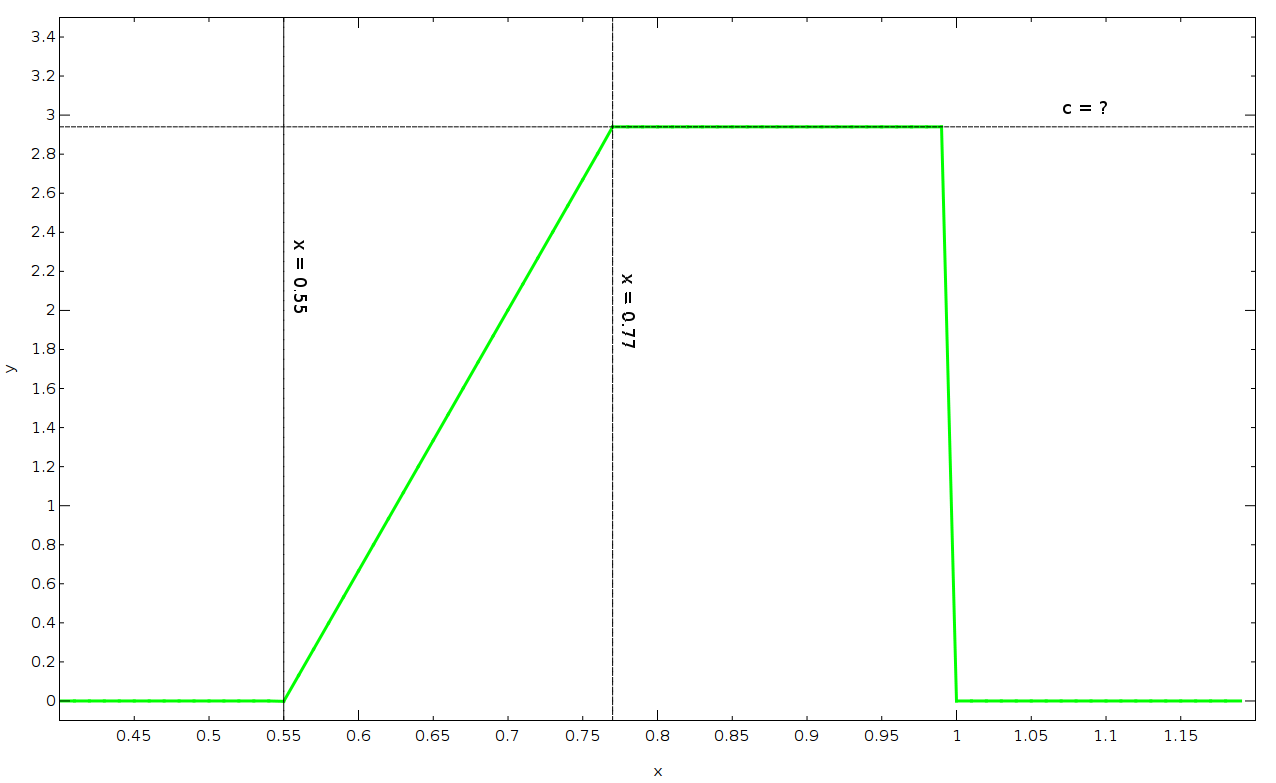
\includegraphics[bb=0 0 700 414 ]{duze.png}
	  \rule{35em}{0.5pt}
	\caption[Wykres kwantyfikatora du�e]{Wykres funkcji g�sto�ci dla kwantyfikatora \emph{du�e}}
	\label{wykres:duze}
\end{figure}
Mamy dany zbi�r punkt�w, przedstawiony na wykresie \ref{wykres:duze}. 
Warto�ci rz�dnych oznaczaj� tutaj warto�� prawdopodbie�stwa natomiast odci�te oznaczaj� stopie� przynale�no�ci prawdopodobie�stwa do kwantyfikatora \emph{du�e}. Przyk�adowo, je�eli m�wimy �e jakie� zdarzenie nast�pi z prawdopodobie�stwem 55\% to nie jest to du�e prawdopodobie�stwo ( prawdopodobie�stwo przynale�y do du�ego prawdopodobie�stwa w stopniu zerowym). Je�li m�wimy natomiast �e jakie� zdarzenie nast�pi z prawdopodobie�stwem 80\% to jest to du�e prawdopodobie�stwo ( stopie� przynale�no�ci jest maksymalny). 
Nasze obliczenia polegaj� na obliczeniu maksymalnego stopnia przynale�no�ci ( maksymalnej warto�ci funkcji g�sto�ci ), co b�dzie stanowi�o wz�r funkcji sta�ej, oraz znalezienia wzoru funkcji liniowej, rozpi�tej mi�dzy punktami o najmniejszym stopniu przynale�no�ci oraz o najwi�kszym stopniu przynale�no�ci. 
Z wykresu odczytujemy punkty graniczne przedzia��w i tak odwzorowania liniowego szukamy na przedziale (0.55,0.77), natomiast sta�ego na przedziale (0.77,1) 
Wynika z tego �e szukana funkcja ma posta�:
\begin{equation}
\label{rownanie:duze_wzor}
f(x) = \left\{ 
\begin{array}{l l}
  ax+b & \quad \text{, for 0.55 $<$ $x$ $\leq$ 0.77}\\
  c & \quad \text{, for 0.77 $<$ $x$ $<$ 1}\\
\end{array} \right.
\end{equation}
Aby znale�� sta�e $a$, $b$ oraz $c$ rozwi�zujemy uk�ad r�wna�:
\begin{equation}
\label{uklad_rownan:duze_ur}
\begin{cases}
(1-0.77)*c + \frac{1}{2}*(0.77-0.55)*c = 1\\
0.55*a + b = 0  \\
0.77*a + b = c \\
\end{cases}
\Rightarrow \;
\begin{cases}
0*a + 0*b + 0.34*c = 1\\
0.55*a + 1*b + 0*c = 0\\
0.77*a + 1*b - 1*c = 0\\
\end{cases}
\end{equation}
Pierwsze r�wanie z uk�adu \ref{uklad_rownan:duze_ur} wynika z faktu, �e funkcja rozk�adu g�sto�ci prawdopodobie�stwa musi si� ca�kowa� do 1 na ca�ym przedziale. (Poza przedzia�em [0.55,1] funkcja jest nieokre�lona, co oznacza, �e pole pod wykresem poza tym przedzia�em jest r�wne 0)
Kolejne dwa  r�wania z uk�adu \ref{uklad_rownan:duze_ur} wynikaj� z rozpi�cia funkcji liniowej mi�dzy punktami (0.55,0) oraz (0.77,$c$). 
Trzecie
Uk�ad r�wna�, przekszta�camy do r�wnania macierzowego:
\begin{equation}
\label{rownanie:duze_macierz}
 \begin{vmatrix} 
 0 & 0 & 0.34 \\ 
 0.55 & 1 & 0 \\
 0.77 & 1 & -1 \\
 \end{vmatrix}
 * 
 \begin{vmatrix} 
 a \\ 
 b \\
 c \\
 \end{vmatrix}
 = 
 \begin{vmatrix} 
 1 \\ 
 0 \\
 0 \\
 \end{vmatrix}
\end{equation} 
co po przekszta�ceniu daje r�wnanie:
\begin{equation}
\label{rownanie:duze_mnozenie_macierzy} 
 \begin{vmatrix} 
 a \\ 
 b \\
 c \\
 \end{vmatrix}
 = 
 {\begin{vmatrix} 
 0 & 0 & 0.34 \\ 
 0.55 & 1 & 0 \\
 0.77 & 1 & -1 \\
 \end{vmatrix}}^{-1}
 *
 \begin{vmatrix} 
 1 \\ 
 0 \\
 0 \\
 \end{vmatrix}
\end{equation} 
Rozwi�zenie tego r�wnania macierzowego istnieje i wynosi 
\begin{equation}
 a = 13.36, 
 b = -7.35,  
 c = 2.94
\end{equation} 
Funkcja rozk�adu g�sto�ci prawdopodobie�stwa, kt�ra aproksymuje zbi�r punkt�w danych dla kwantyfikatora \emph{du�e} wygl�da zatem nast�puj�co:
\begin{equation}
\label{rownanie:duze_wynik}
f(x) = \left\{ 
\begin{array}{l l}
  13.36x - 7.35 & \quad \text{, for 0.55 $<$ $x$ $\leq$ 0.77}\\
  2.94 & \quad \text{, for 0.77 $<$ $x$ $<$ 1}\\
\end{array}\right.
\end{equation}

\subsection{Kwantyfikator "ma�e"}
Funkcje g�sto�ci dla kwantyfikatora \emph{ma�e}, kt�rego rozk�ad pokazuje wykres otrzymujemy w analogiczny spos�b jak dla kwantyfikatora \emph{du�e}. 
\begin{figure}[htbp]
	\label{fig:wykres_male}
	\centering
	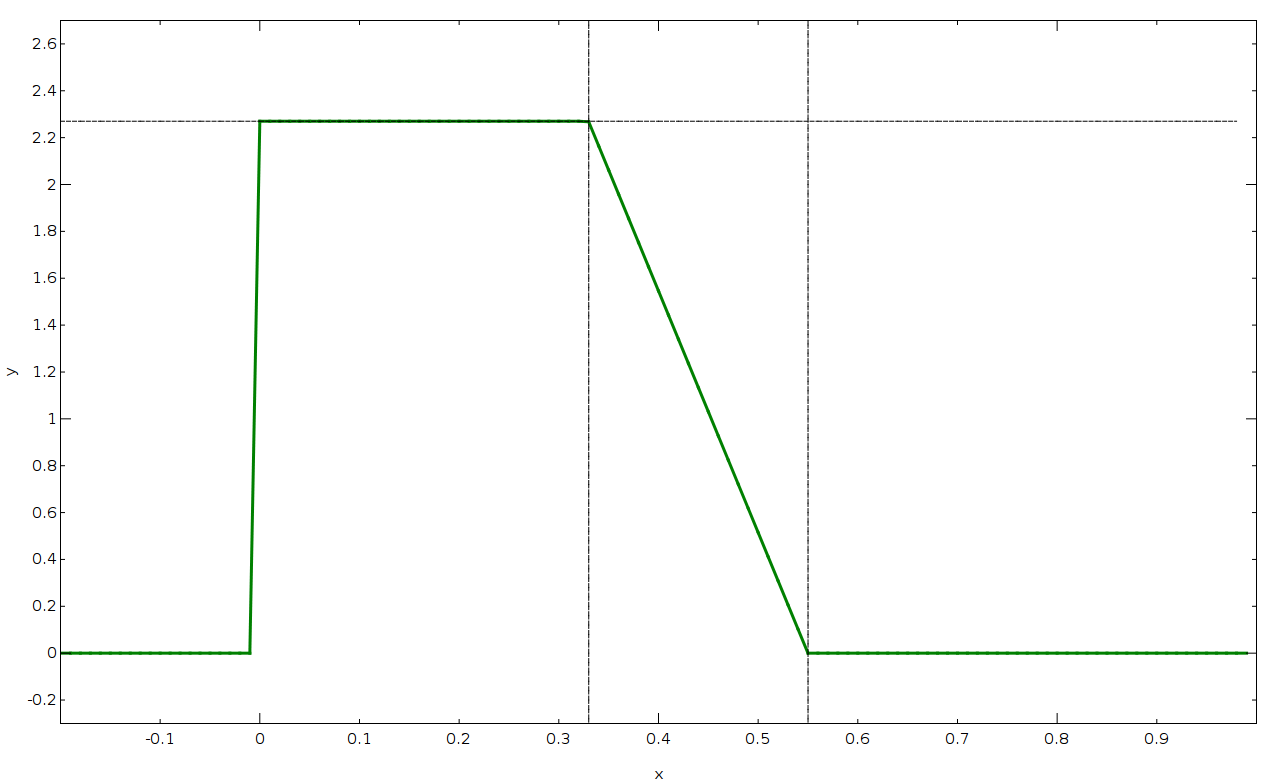
\includegraphics[bb=0 0 800 505 ]{male.png}
	  \rule{35em}{0.5pt}
	\caption[Wykres kwantyfikatora ma�e]{Wykres funkcji g�sto�ci dla kwantyfikatora \emph{ma�e}}
\end{figure}
Funkcja ta jest postaci podobnej do funkcji opisanej wzorem \ref{rownanie:duze_wzor} : 
\begin{equation}
\label{rownanie:male_wzor}
f(x) = \left\{ 
\begin{array}{l l}
  ax+b & \quad \text{, for 0.33 $<$ $x$ $\leq$ 0.55}\\
  c & \quad \text{, for 0 $<$ $x$ $<$ 0.33}\\
\end{array} \right.
\end{equation}
Aby obliczy� $a$, $b$ oraz $c$ rozwi�zujemy uk�ad analogiczny do uk�adu r�wna� \ref{uklad_rownan:duze_ur}. 
Ko�cowe operacja jest analogiczna do mno�enia macierzy \ref{rownanie:duze_mnozenie_macierzy}, i wygl�da nast�puj�co:
\begin{equation}
\label{rownanie:male_mnozenie_macierzyy} 
 \begin{vmatrix} 
 a \\ 
 b \\
 c \\
 \end{vmatrix}
 = 
 {\begin{vmatrix} 
 0 & 0 & 0.44 \\ 
 0.55 & 1 & 0 \\
 0.33 & 1 & -1 \\
 \end{vmatrix}}^{-1}
 *
 \begin{vmatrix} 
 1 \\ 
 0 \\
 0 \\
 \end{vmatrix}
\end{equation} 
Rozwi�zanie tego uk�adu wygl�da nast�puj�co:
\begin{equation}
 a = -10.33, 
 b = 5.68,  
 c = 2.27
\end{equation} 
Funkcja rozk�adu g�sto�ci prawdopodobie�stwa, kt�ra aproksymuje zbi�r punkt�w danych dla kwantyfikatora \emph{ma�e} wygl�da zatem nast�puj�co:

\begin{equation}
\label{rownanie:male_wynik}
f(x) = \left\{ 
\begin{array}{l l}
  -10.31*x + 5.67 & \quad \text{, for 0.33 $<$ $x$ $\leq$ 0.55}\\
  2.27 & \quad \text{, for 0 $<$ $x$ $<$ 0.33}\\
\end{array} \right.
\end{equation}

\subsection{Kwantyfikator "bliskie 10 mln"}
Kwantyfikator \emph{bliskie 10 mln} jest zadany przez wykres funkcji \ref{wykres:bliskie10mln}. 
\begin{figure}[htbp]
	\centering
	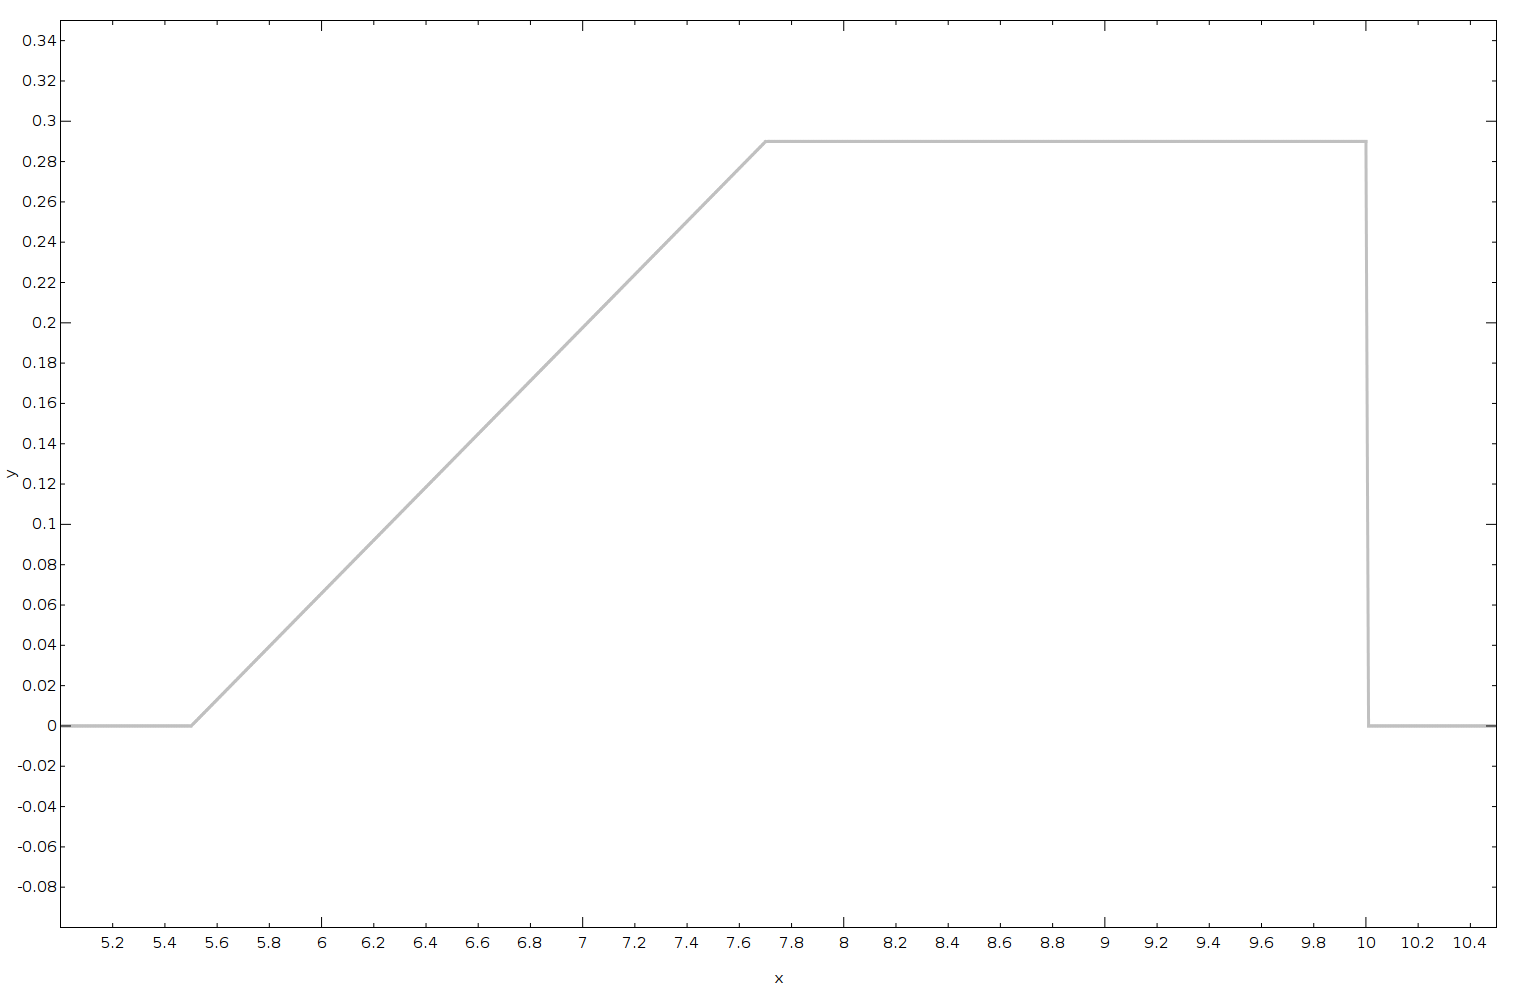
\includegraphics[bb=0 0 700 462 ]{bliskie10mln.png}
	  \rule{35em}{0.5pt}
	\caption[Wykres kwantyfikatora bliskie 10 mln]{Wykres funkcji g�sto�ci dla kwantyfikatora  \emph{bliskie 10 mln}}
      \label{wykres:bliskie10mln}
\end{figure}
Tym razem, kwantyfikator ten nie jest wynikiem ankiety, tylko jest zadany przez Profesora Piegata( to samo tyczy si� pozosta�em 
Aby uzyska� wz�r funkcji dla tego i reszty kwantyfikator�w, rozwi�zujemy uk�ad r�wna� analogiczny do uk�adu \ref{uklad_rownan:duze_ur} o postaci:
\begin{equation}
\label{bliskie10mln_uklad_rownan}
\begin{cases}
(10 - 7.7)*c + \frac{1}{2}*(7.7-5.5)*c = 1\\
5.5*a + b = 0  \\
7.7*a + b = c \\
\end{cases}
\end{equation}
Ko�cowa operacja macierzowa wygl�da nast�puj�co:
\begin{equation}
\label{male_mnozenie_macierzy} 
 \begin{vmatrix} 
 a \\ 
 b \\
 c \\
 \end{vmatrix}
 = 
 {\begin{vmatrix} 
 0 & 0 & 3.4 \\ 
 5.5 & 1 & 0 \\
 7.7 & 1 & -1 \\
 \end{vmatrix}}^{-1}
 *
 \begin{vmatrix} 
 1 \\ 
 0 \\
 0 \\
 \end{vmatrix}
\end{equation} 
Rozwi�zanie tego uk�adu wygl�da nast�puj�co:
\begin{equation}
 a = 0.13, 
 b = -0.73,  
 c = 0.29
\end{equation} 
Funkcja rozk�adu g�sto�ci prawdopodobie�stwa, kt�ra aproksymuje zbi�r punkt�w danych dla kwantyfikatora  \emph{bliskie 10 mln} wygl�da zatem nast�puj�co:

\begin{equation}
\label{equation_male_wynik}
f(x) = \left\{ 
\begin{array}{l l}
  0.13*x - 0.73 & \quad \text{, for 5.5 $<$ $x$ $\leq$ 7.7}\\
  0.29 & \quad \text{, for 7.7 $<$ $x$ $<$ 1}\\
\end{array} \right.
\end{equation}


\subsection{Kwantyfikator "nie bliskie 10 mln"}
Kwantyfikator \emph{nie bliskie 10 mln} jest zadany przez wykres funkcji \ref{wykres:niebliskie10mln}. 
\begin{figure}[htbp]
	
	\centering
	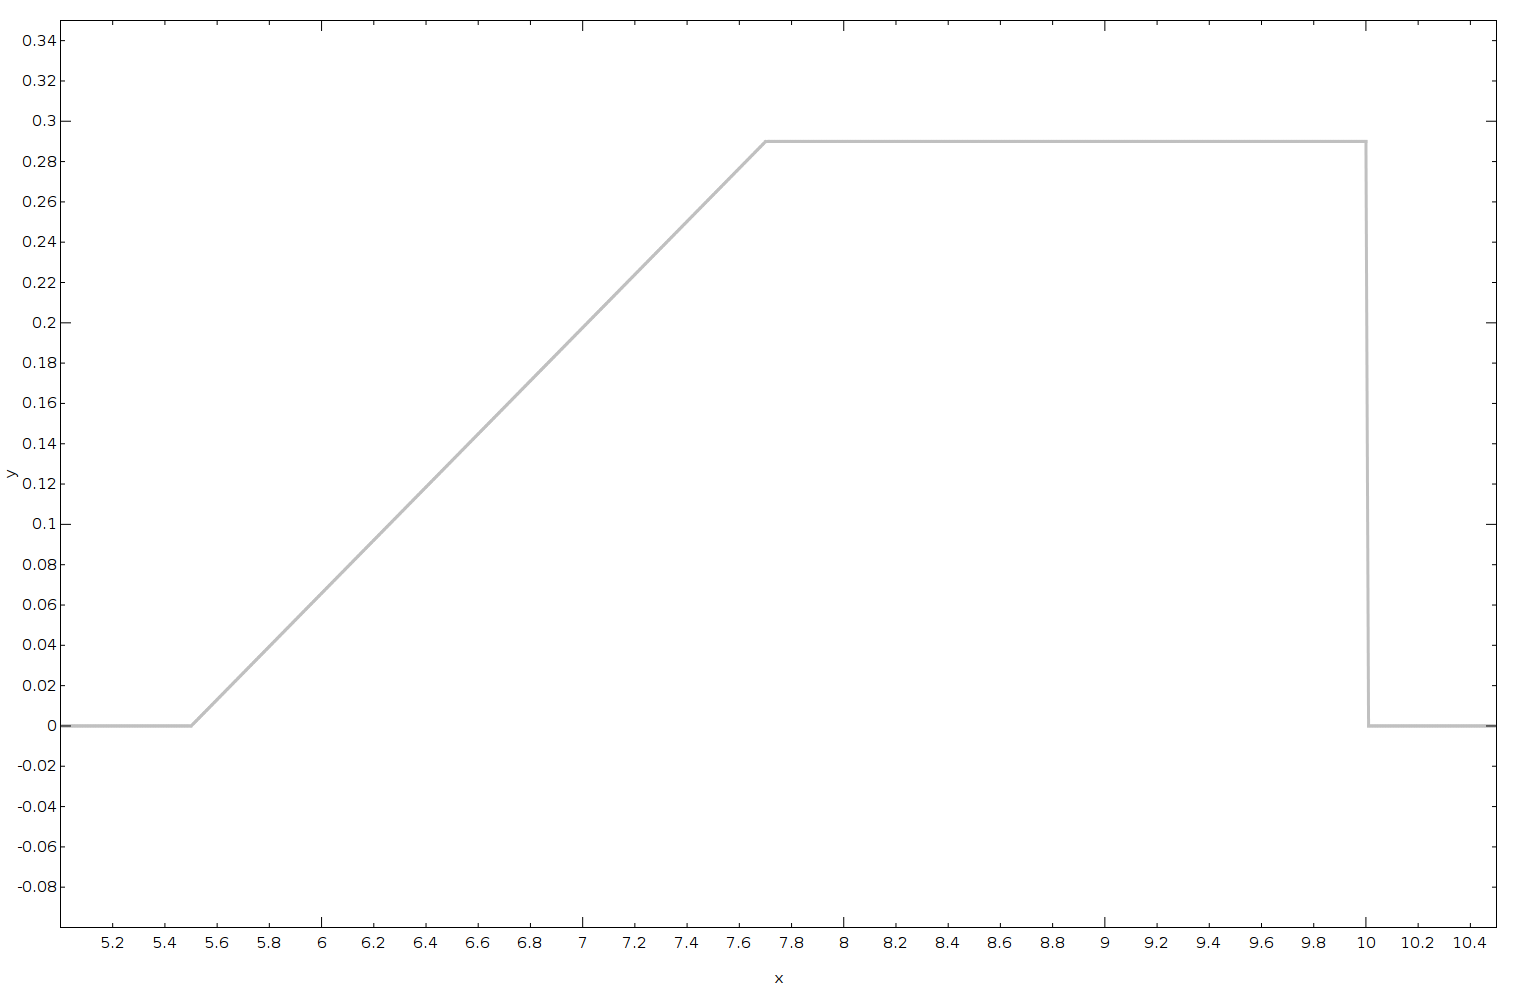
\includegraphics[bb=0 0 700 462 ]{bliskie10mln.png}
	  \rule{35em}{0.5pt}
	\caption[Wykres kwantyfikatora bliskie 10 mln]{Wykres funkcji g�sto�ci dla kwantyfikatora \emph{nie bliskie 10 mln}}
	\label{wykres:niebliskie10mln}
\end{figure}
Aby uzyska� wz�r funkcji dla tego i reszty kwantyfikator�w, rozwi�zujemy uk�ad r�wna� analogiczny do uk�adu \ref{uklad_rownan:duze_ur} o postaci
\begin{equation}
\label{niebliskie10mln_uklad_rownan}
\begin{cases}
5.5*c + \frac{1}{2}*(7.7-5.5)*c = 1\\
5.5*a + b = c  \\
7.7*a + b = 0 \\
\end{cases}
\end{equation}
Finalna operacja macierzowa wygl�da nast�puj�co:
\begin{equation}
\label{male_mnozenie_macierzy} 
 \begin{vmatrix} 
 a \\ 
 b \\
 c \\
 \end{vmatrix}
 = 
 {\begin{vmatrix} 
 0 & 0 & 6.6 \\ 
 5.5 & 1 & -1 \\
 7.7 & 1 & 0 \\
 \end{vmatrix}}^{-1}
 *
 \begin{vmatrix} 
 1 \\ 
 0 \\
 0 \\
 \end{vmatrix}
\end{equation} 
Rozwi�zanie tego uk�adu wygl�da nast�puj�co:
\begin{equation}
 a = -0.06, 
 b = 0.53,  
 c = 0.15
\end{equation} 
Funkcja rozk�adu g�sto�ci prawdopodobie�stwa, kt�ra aproksymuje zbi�r punkt�w danych dla kwantyfikatora  \emph{nie bliskie 10 mln} wygl�da zatem nast�puj�co:

\begin{equation}
\label{equation_male_wynik}
f(x) = \left\{ 
\begin{array}{l l}
 -0.06*x +  0.53 & \quad \text{, for 5.5 $<$ $x$ $\leq$ 7.7}\\
  0.15 & \quad \text{, for 0 $<$ $x$ $<$ 5.5}\\
\end{array} \right.
\end{equation}
\subsection{Kwantyfikator "bliskie 20 mln"}
Kwantyfikator \emph{bliskie 20 mln} jest zadany przez wykres funkcji \ref{wykres:bliskie20mln}. 
\begin{figure}[htbp]
  
    \centering
    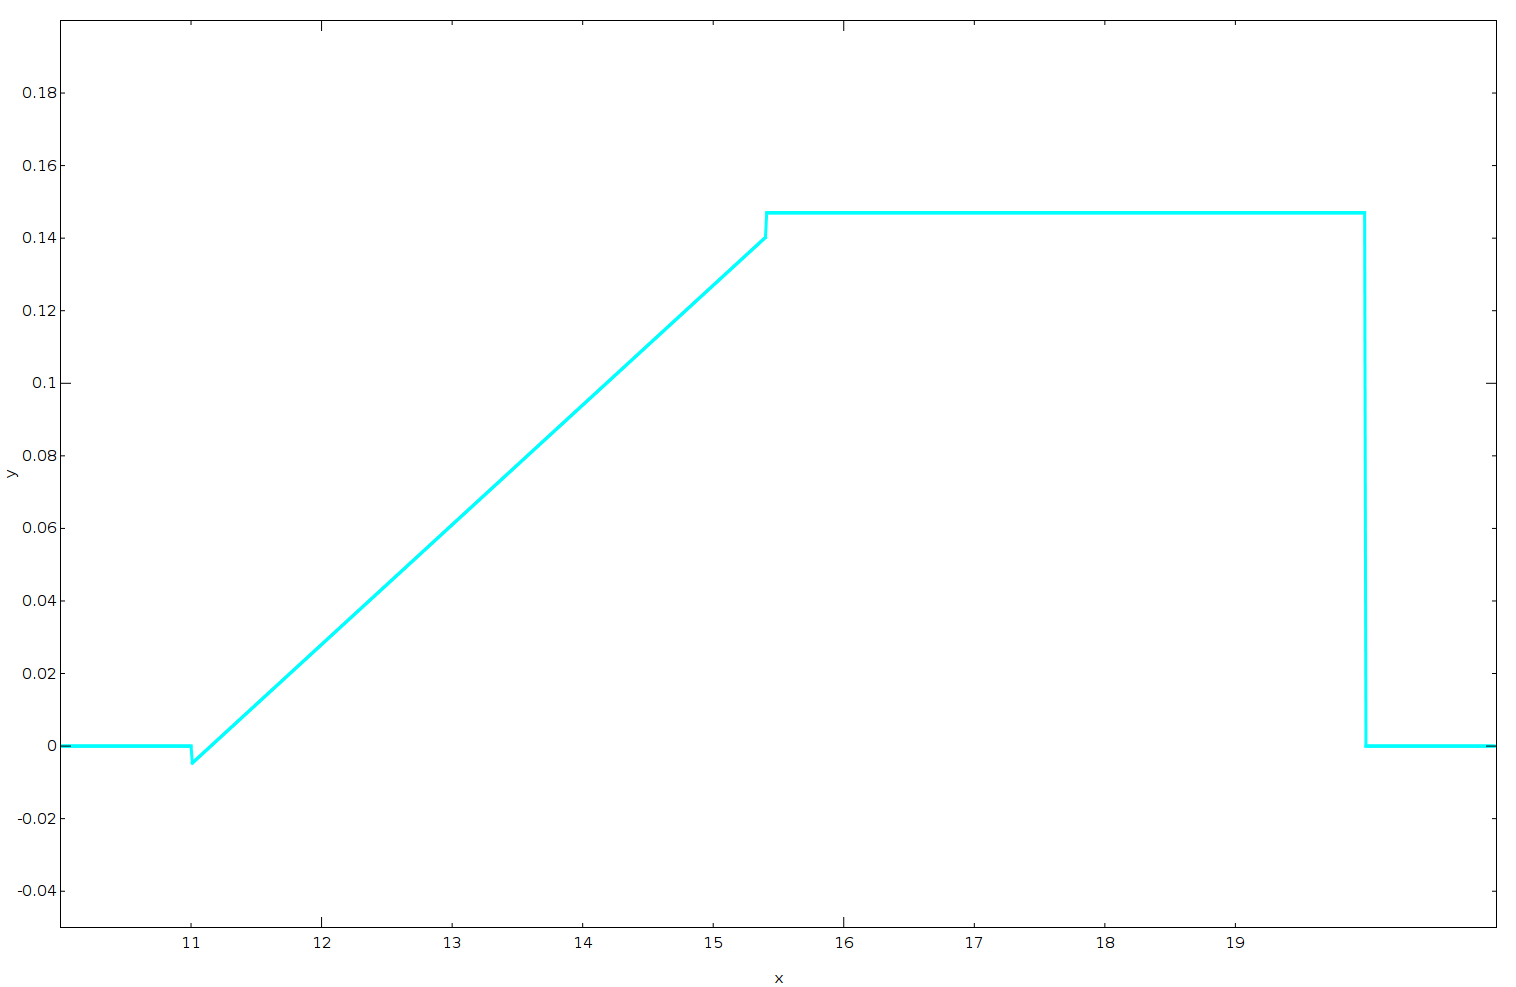
\includegraphics[bb=0 0 700 462 ]{bliskie20mln.png}
        \rule{35em}{0.5pt}
    \caption[Wykres kwantyfikatora bliskie 10 mln]{Wykres funkcji g�sto�ci dla kwantyfikatora \emph{nie bliskie 10 mln}}
    \label{wykres:bliskie20mln}
\end{figure}
Aby uzyska� wz�r funkcji dla tego i reszty kwantyfikator�w, rozwi�zujemy uk�ad r�wna� analogiczny do uk�adu \ref{uklad_rownan:duze_ur} o postaci
\begin{equation}
\label{bliskie20mln_uklad_rownan}
\begin{cases}
(20-15.4)*c + \frac{1}{2}*(15.4-11)*c = 1\\
11*a + b = 0  \\
15.4*a + b = c \\
\end{cases}
\end{equation}
Finalna operacja macierzowa wygl�da nast�puj�co:
\begin{equation}
\label{bliskie20_mnozenie_macierzy} 
 \begin{vmatrix} 
 a \\ 
 b \\
 c \\
 \end{vmatrix}
 = 
 {\begin{vmatrix} 
 0 & 0 & 11 \\ 
 11 & 1 & 0 \\
 15.4 & 1 & -1 \\
 \end{vmatrix}}^{-1}
 *
 \begin{vmatrix} 
 1 \\ 
 0 \\
 0 \\
 \end{vmatrix}
\end{equation} 
Rozwi�zanie tego uk�adu wygl�da nast�puj�co:
\begin{equation}
 a = 0.02, 
 b = -0.22,  
 c = 0.09
\end{equation} 
Funkcja rozk�adu g�sto�ci prawdopodobie�stwa, kt�ra aproksymuje zbi�r punkt�w danych dla kwantyfikatora  \emph{bliskie 20 mln} wygl�da zatem nast�puj�co:
\begin{equation}
\label{equation_bliskie20_wynik}
f(x) = \left\{ 
\begin{array}{l l}
 0.02*x -  0.22 & \quad \text{, for 11 $<$ $x$ $\leq$ 15.4}\\
  0.09 & \quad \text{, for 15.4 $<$ $x$ $<$ 20}\\
\end{array} \right.
\end{equation}

\subsection{Kwantyfikator "nie bliskie 20 mln"}

Poni�ej, pokazano parami, funkcje rozk�adu g�sto�ci prawdopodobni�stwa dla kwantyfikator�w. Na jednym wykresie zawarto kwantyfikator wraz z kwantyfikatorem do niego przeciwnym. 

\todo{Doda� rysunki kwantyfikator�w parami}%

% \begin{figure}[htbp]
%   
%     \centering
%     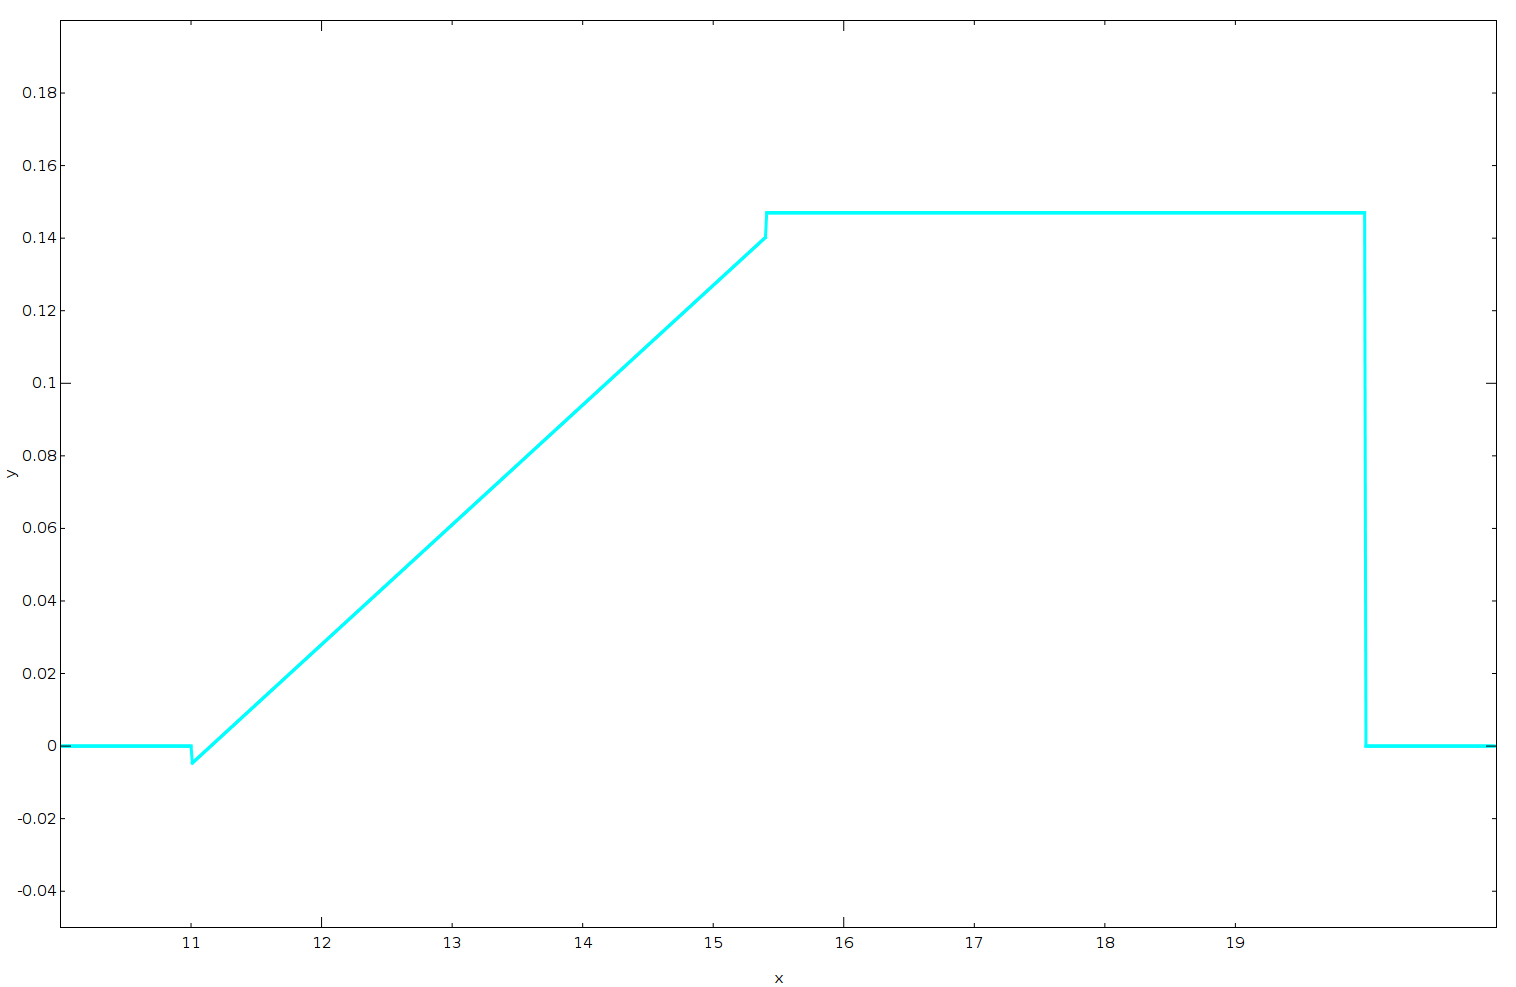
\includegraphics[bb=0 0 700 462 ]{bliskie20mln.png}
%         \rule{35em}{0.5pt}
%     \caption[Wykres kwantyfikatora bliskie 10 mln]{Wykres funkcji g�sto�ci dla kwantyfikatora \emph{nie bliskie 10 mln}}
%     \label{wykres:bliskie20mln}
% \end{figure}



\section{Rozwi�zanie problemu}
 % Experiment 1

%\input{./Chapters/Chapter5} % Experiment 2

%\input{./Chapters/Chapter6} % Results and Discussion

%\input{./Chapters/Chapter7} % Conclusion

%% ----------------------------------------------------------------
% Now begin the Appendices, including them as separate files

\addtocontents{toc}{\vspace{2em}} % Add a gap in the Contents, for aesthetics

\appendix % Cue to tell LaTeX that the following 'chapters' are Appendices

% Appendix A

\chapter{Appendix Title Here}
\label{AppendixA}
\lhead{Appendix A. \emph{Appendix Title Here}}

Write your Appendix content here.	% Appendix Title

%\input{./Appendices/AppendixB} % Appendix Title

%\input{./Appendices/AppendixC} % Appendix Title

\addtocontents{toc}{\vspace{2em}}  % Add a gap in the Contents, for aesthetics
\backmatter

%% ----------------------------------------------------------------
\label{Bibliography}
\lhead{\emph{Bibliography}}  % Change the left side page header to "Bibliography"
\bibliographystyle{unsrtnat}  % Use the "unsrtnat" BibTeX style for formatting the Bibliography
\bibliography{Bibliography}  % The references (bibliography) information are stored in the file named "Bibliography.bib"

\end{document}  % The End
%% ----------------------------------------------------------------
